\documentclass{mpaper}
\usepackage{xparse}
\usepackage{mathtools}

\usepackage{tikz}
%\usepackage{pgfplots}
\usetikzlibrary{fit, arrows.meta, calc}
\usepackage{gnuplot-lua-tikz}
%\usepgfplotslibrary{external} 
%\tikzexternalize

\usepackage[binary-units]{siunitx}
\sisetup{range-phrase=--, range-units=single}

\usepackage{lipsum}
\usepackage[basic]{complexity}
\usepackage[super,negative]{nth}

\usepackage[linesnumbered,vlined,ruled,commentsnumbered]{algorithm2e}
\SetNlSty{}{}{}
\SetAlgoNlRelativeSize{-3}

\usepackage[labelfont=bf,textfont={bf,it}]{caption}
\usepackage{subcaption}
\captionsetup[subfigure]{justification=centering}
\usepackage{cleveref}
\newcommand{\crefrangeconjunction}{--}
\usepackage{enumitem}
%\setlist{nosep}
\usepackage[mode=buildmissing]{standalone}
\usepackage{booktabs}
\usepackage{microtype}

\usepackage[backend=bibtex,maxnames=3,maxbibnames=99,style=trad-abbrv]{biblatex}
\addbibresource{mprop.bib}

% Addendum formatting (thanks, http://tex.stackexchange.com/questions/339471/indented-addendums-using-biblatex-sourcemaps)
% Also remove doi, url since unnecessary
\DeclareFieldFormat{addendum}{}
%\DeclareFieldFormat{url}{}
%\DeclareFieldFormat{doi}{}
\DeclareFieldFormat*{url}{}
\DeclareFieldFormat[online]{url}{\mkbibacro{URL}\addcolon\space\url{#1}}
%\DeclareFieldFormat*{urldate}{}
%\DeclareFieldFormat[online]{urldate}{\mkbibparens{\bibstring{urlseen}\space#1}}

\usepackage{xpatch}

\xpatchbibmacro{name:andothers}{%
	\bibstring{andothers}%
}{%
	\bibstring[\emph]{andothers}%
}{}{}

\definecolor{graphc1}{RGB}{150,227,240}
\definecolor{graphc2}{RGB}{250,71,37}
\definecolor{graphc3}{RGB}{253,161,77}
\definecolor{graphc4}{RGB}{141,246,135}

% Official colours!

\definecolor{uofguniversityblue}{rgb}{0, 0.219608, 0.396078}

\definecolor{uofgheather}{rgb}{0.356863, 0.32549, 0.490196}
\definecolor{uofgaquamarine}{rgb}{0.603922, 0.72549, 0.678431}
\definecolor{uofgslate}{rgb}{0.309804, 0.34902, 0.380392}
\definecolor{uofgrose}{rgb}{0.823529, 0.470588, 0.709804}
\definecolor{uofgmocha}{rgb}{0.709804, 0.564706, 0.47451}

\definecolor{uofglawn}{rgb}{0.517647, 0.741176, 0}
\definecolor{uofgcobalt}{rgb}{0, 0.615686, 0.92549}
\definecolor{uofgturquoise}{rgb}{0, 0.709804, 0.819608}
\definecolor{uofgsunshine}{rgb}{1.0, 0.862745, 0.211765}
\definecolor{uofgpumpkin}{rgb}{1.0, 0.72549, 0.282353}
\definecolor{uofgthistle}{rgb}{0.584314, 0.070588, 0.447059}
\definecolor{uofgpillarbox}{rgb}{0.701961, 0.047059, 0}
\definecolor{uofglavendar}{rgb}{0.356863, 0.301961, 0.580392}

\definecolor{uofgsandstone}{rgb}{0.321569, 0.278431, 0.231373}
\definecolor{uofgforest}{rgb}{0, 0.317647, 0.2}
\definecolor{uofgburgundy}{rgb}{0.490196, 0.133333, 0.223529}
\definecolor{uofgrust}{rgb}{0.603922, 0.227451, 0.023529}

\newcommand{\lesspreceq}[1]{\prescript{}{#1}{\preceq}\ }

% Custom headings, sweet!
\newcommand{\subparagraph}{}
\usepackage[uppercase,tiny,noindentafter]{titlesec}
\titleformat{\subsection}{\normalfont\bfseries}{\thesubsection.}{1em}{}
\titleformat{\subsubsection}{\normalfont\bfseries}{\thesubsubsection.}{1em}{}
\titlelabel{\thetitle.\quad}
\titleformat{\paragraph}[runin]{\normalfont\normalsize\bfseries}{\theparagraph}{1em}{}

\begin{document}

\title{Graph Models and Maximum Common Subgraph for Character Analysis}
\author{Kyle A. Simpson}
\matricnum{2029567}

\maketitle
%====================================================
%====================================================
\begin{abstract}
According to Simon Peyton Jones, an abstract should address
four key questions. First, what is the problem that this
paper tackles? Second, why is this an interesting problem?
Third, what is the solution this paper proposes?
Finally, why is the proposed solution a good one?
%Lorem ipsum dolor sit amet lorem ipsum dolor sit amet lorem ipsum dolor sit amet lorem ipsum dolor sit amet lorem ipsum dolor sit amet lorem ipsum dolor sit amet lorem ipsum dolor sit amet lorem ipsum dolor sit amet lorem ipsum dolor sit amet lorem ipsum dolor sit amet lorem ipsum dolor sit amet lorem ipsum dolor sit amet lorem ipsum dolor sit amet lorem ipsum dolor sit amet lorem ipsum dolor sit amet lorem ipsum dolor sit amet lorem ipsum dolor sit amet lorem ipsum dolor sit amet lorem ipsum dolor sit amet lorem ipsum dolor sit amet lorem ipsum dolor sit amet
%\lipsum[1]

?? Write me
\end{abstract}
%====================================================
%====================================================

%====================================================
\section{Introduction}
\label{sec:introduction}
%====================================================

%?? Adapt proposal introduction
Research into computer vision tasks, such as image and object recognition, is currently dominated by the use of machine learning and vector-space models, while graph encodings are comparatively less well-explored.
%Neural networks and similar machine learning constructs learn features of the inputs and data they are given, which are later used to classify or identify patterns in images or generic datasets---and have become popular due to their versatility, effectiveness and accuracy across many problem domains.
Machine learning methods typically rely on these vector-space models, applying statistical inference from training data to teach classifiers how to recognise the desired elements or features from an image---and have become popular due to their versatility, effectiveness and accuracy across many problem domains.
Some of these vector-space models take a \emph{keypoint} approach, capturing the area around high-contrast regions in images as salient features, or might examine \emph{codings} which describe an image's contents in a dense and very low-level fashion.

In many cases it can be hard to reason about such models' robustness or sensitivity to different phenomena.
In a machine learning context, for instance, these are often a function of both the training data and the model itself.
The parameters learned by these models aren't structured in a way that allows humans to easily intuit what the model has learned or to comment on the system's correctness, and it can be difficult to discern \textit{why} a particular image might be misclassified.
Recent work into \emph{adversarial images} \cite{AdversarialML} has confirmed this, given that interference can lead to classifications contrary to image content.
%Outside of this, vector-space models can represent image interest points in a way that describes their neighbourhood (or indeed, the entirety of an image), and so are easier to understand; yet they lack any way to describe the relationships between these points or to capture an object's shape.

%?? Adversarial examples in ML \cite{AdversarialML}

\begin{figure}[ht]
	\centering
	\resizebox{\columnwidth}{!}{
		\Large
		\begin{tikzpicture}
		\node[inner sep=5pt] (sagrada1) at (0,0)
		{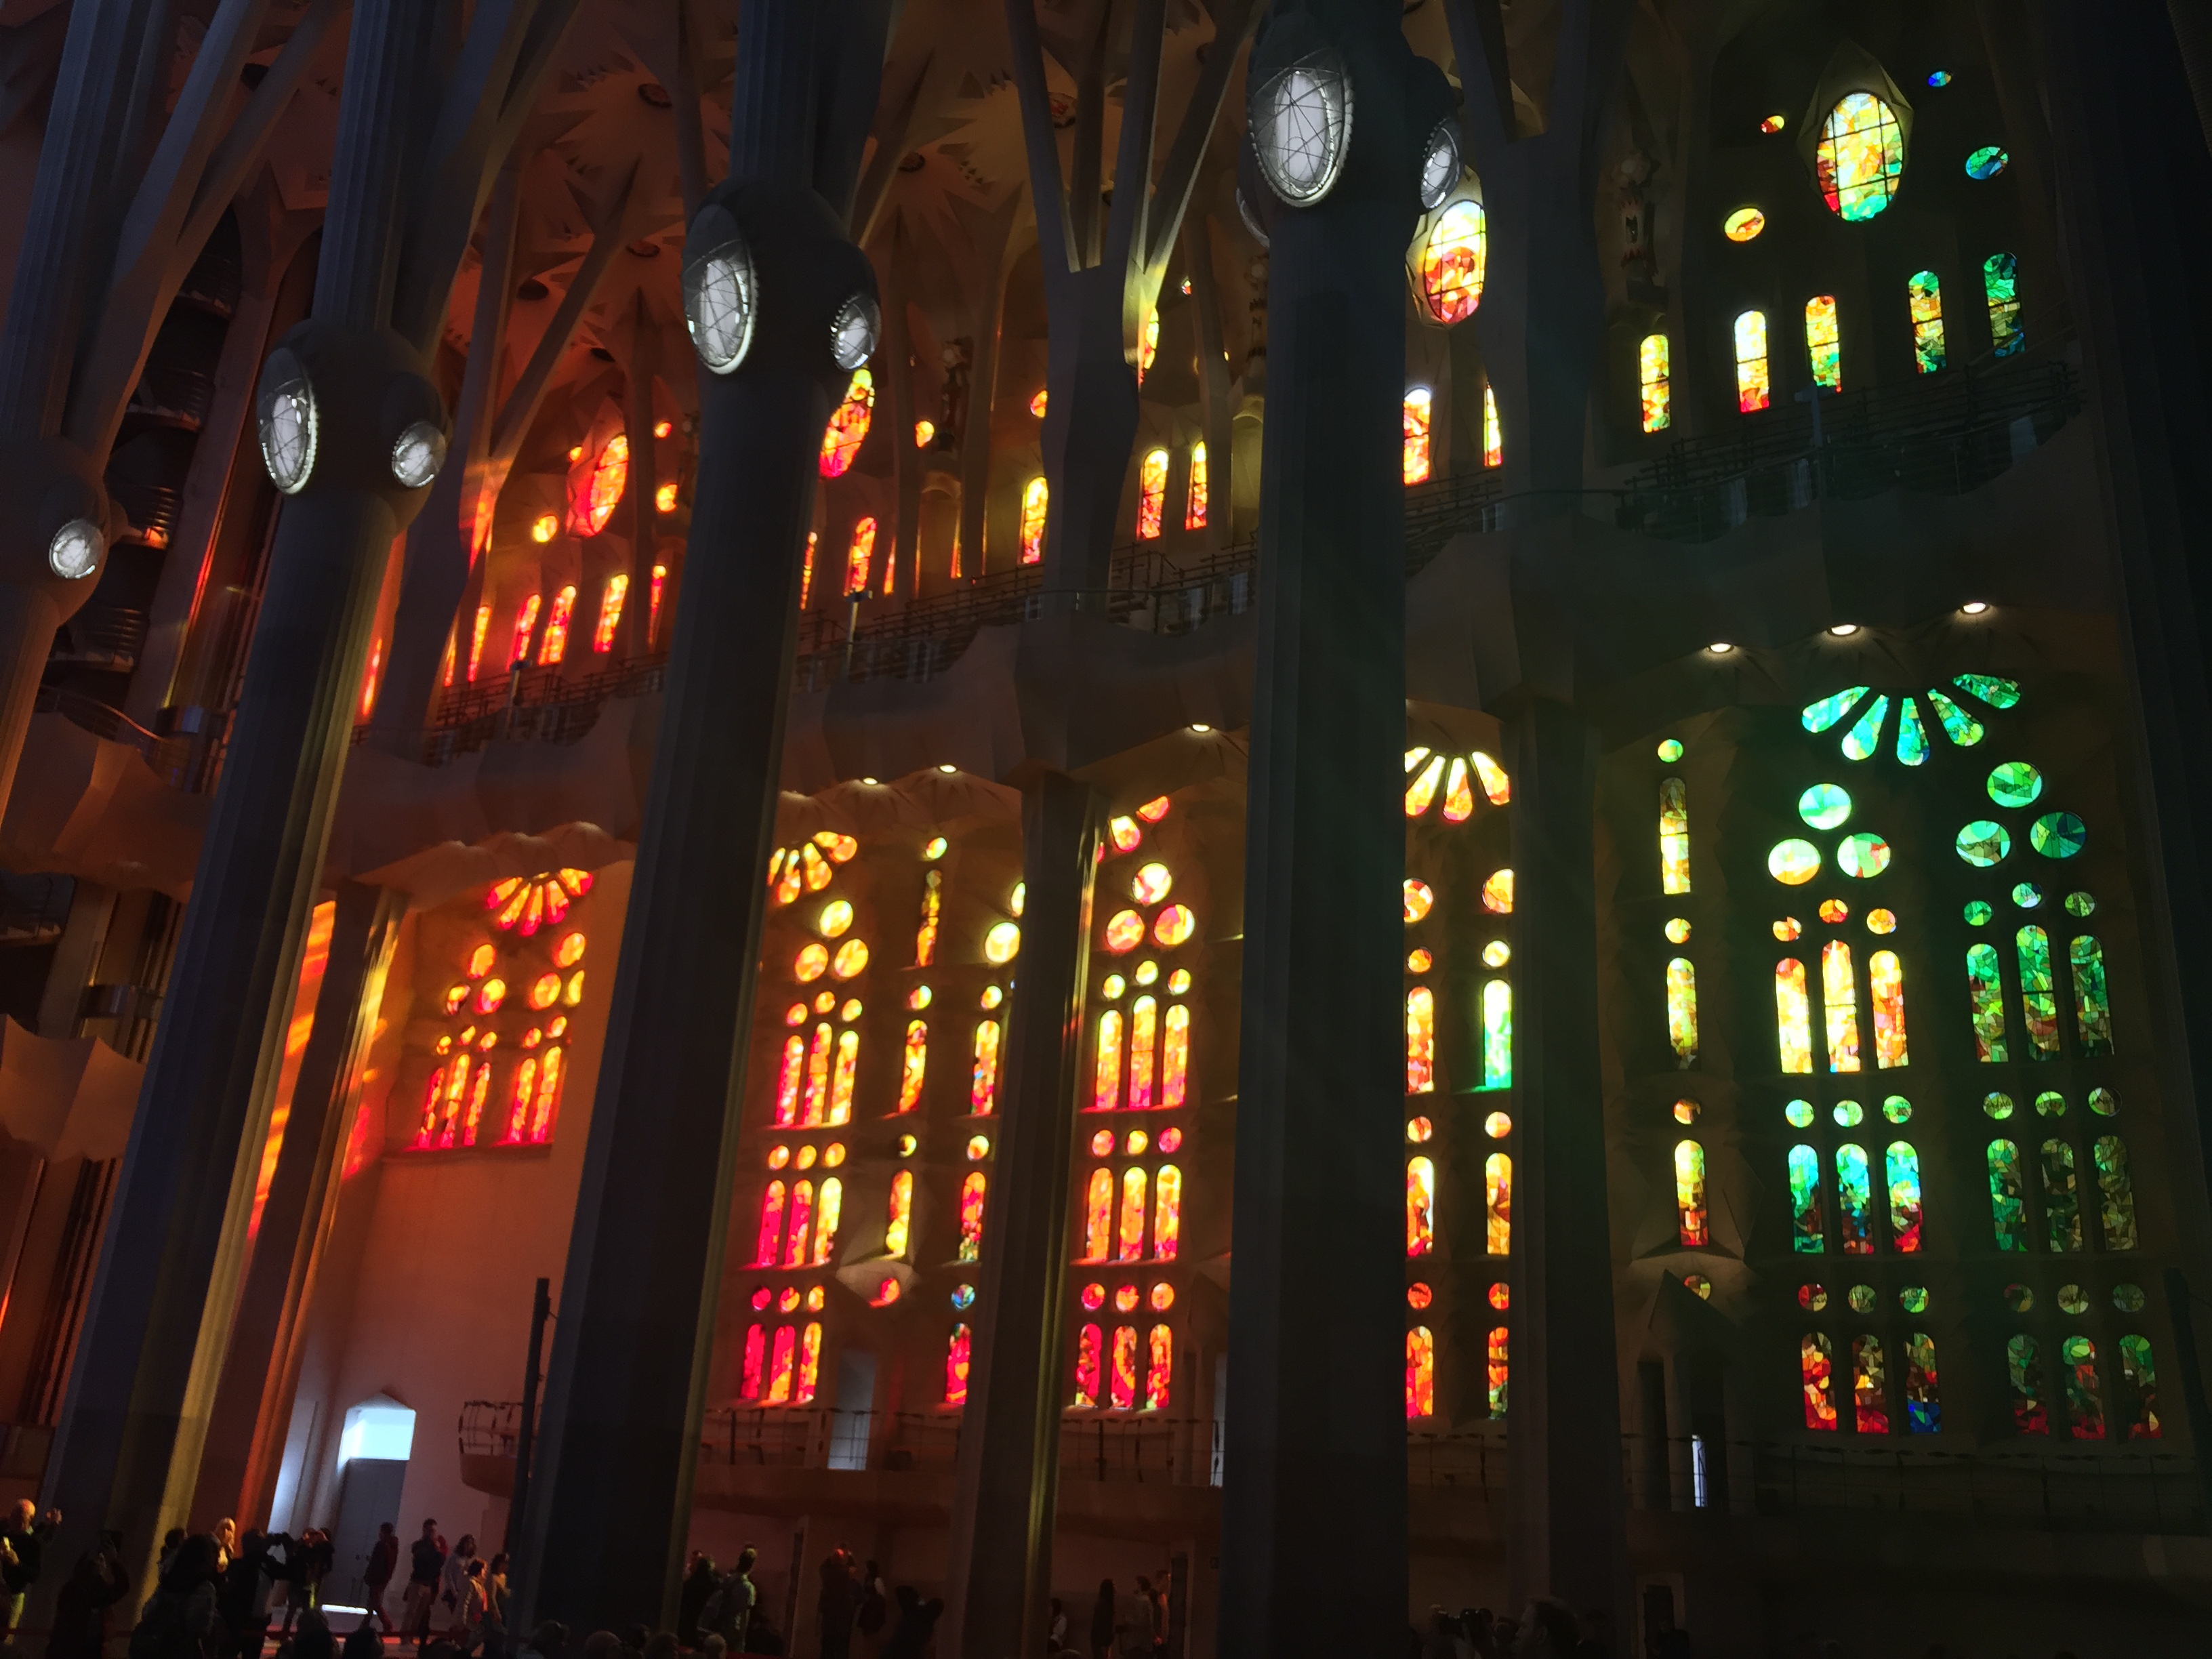
\includegraphics[width=.35\textwidth]{images/IMG_3267.JPG}};
		\node[inner sep=5pt] (sagrada2) at (10,0)
		{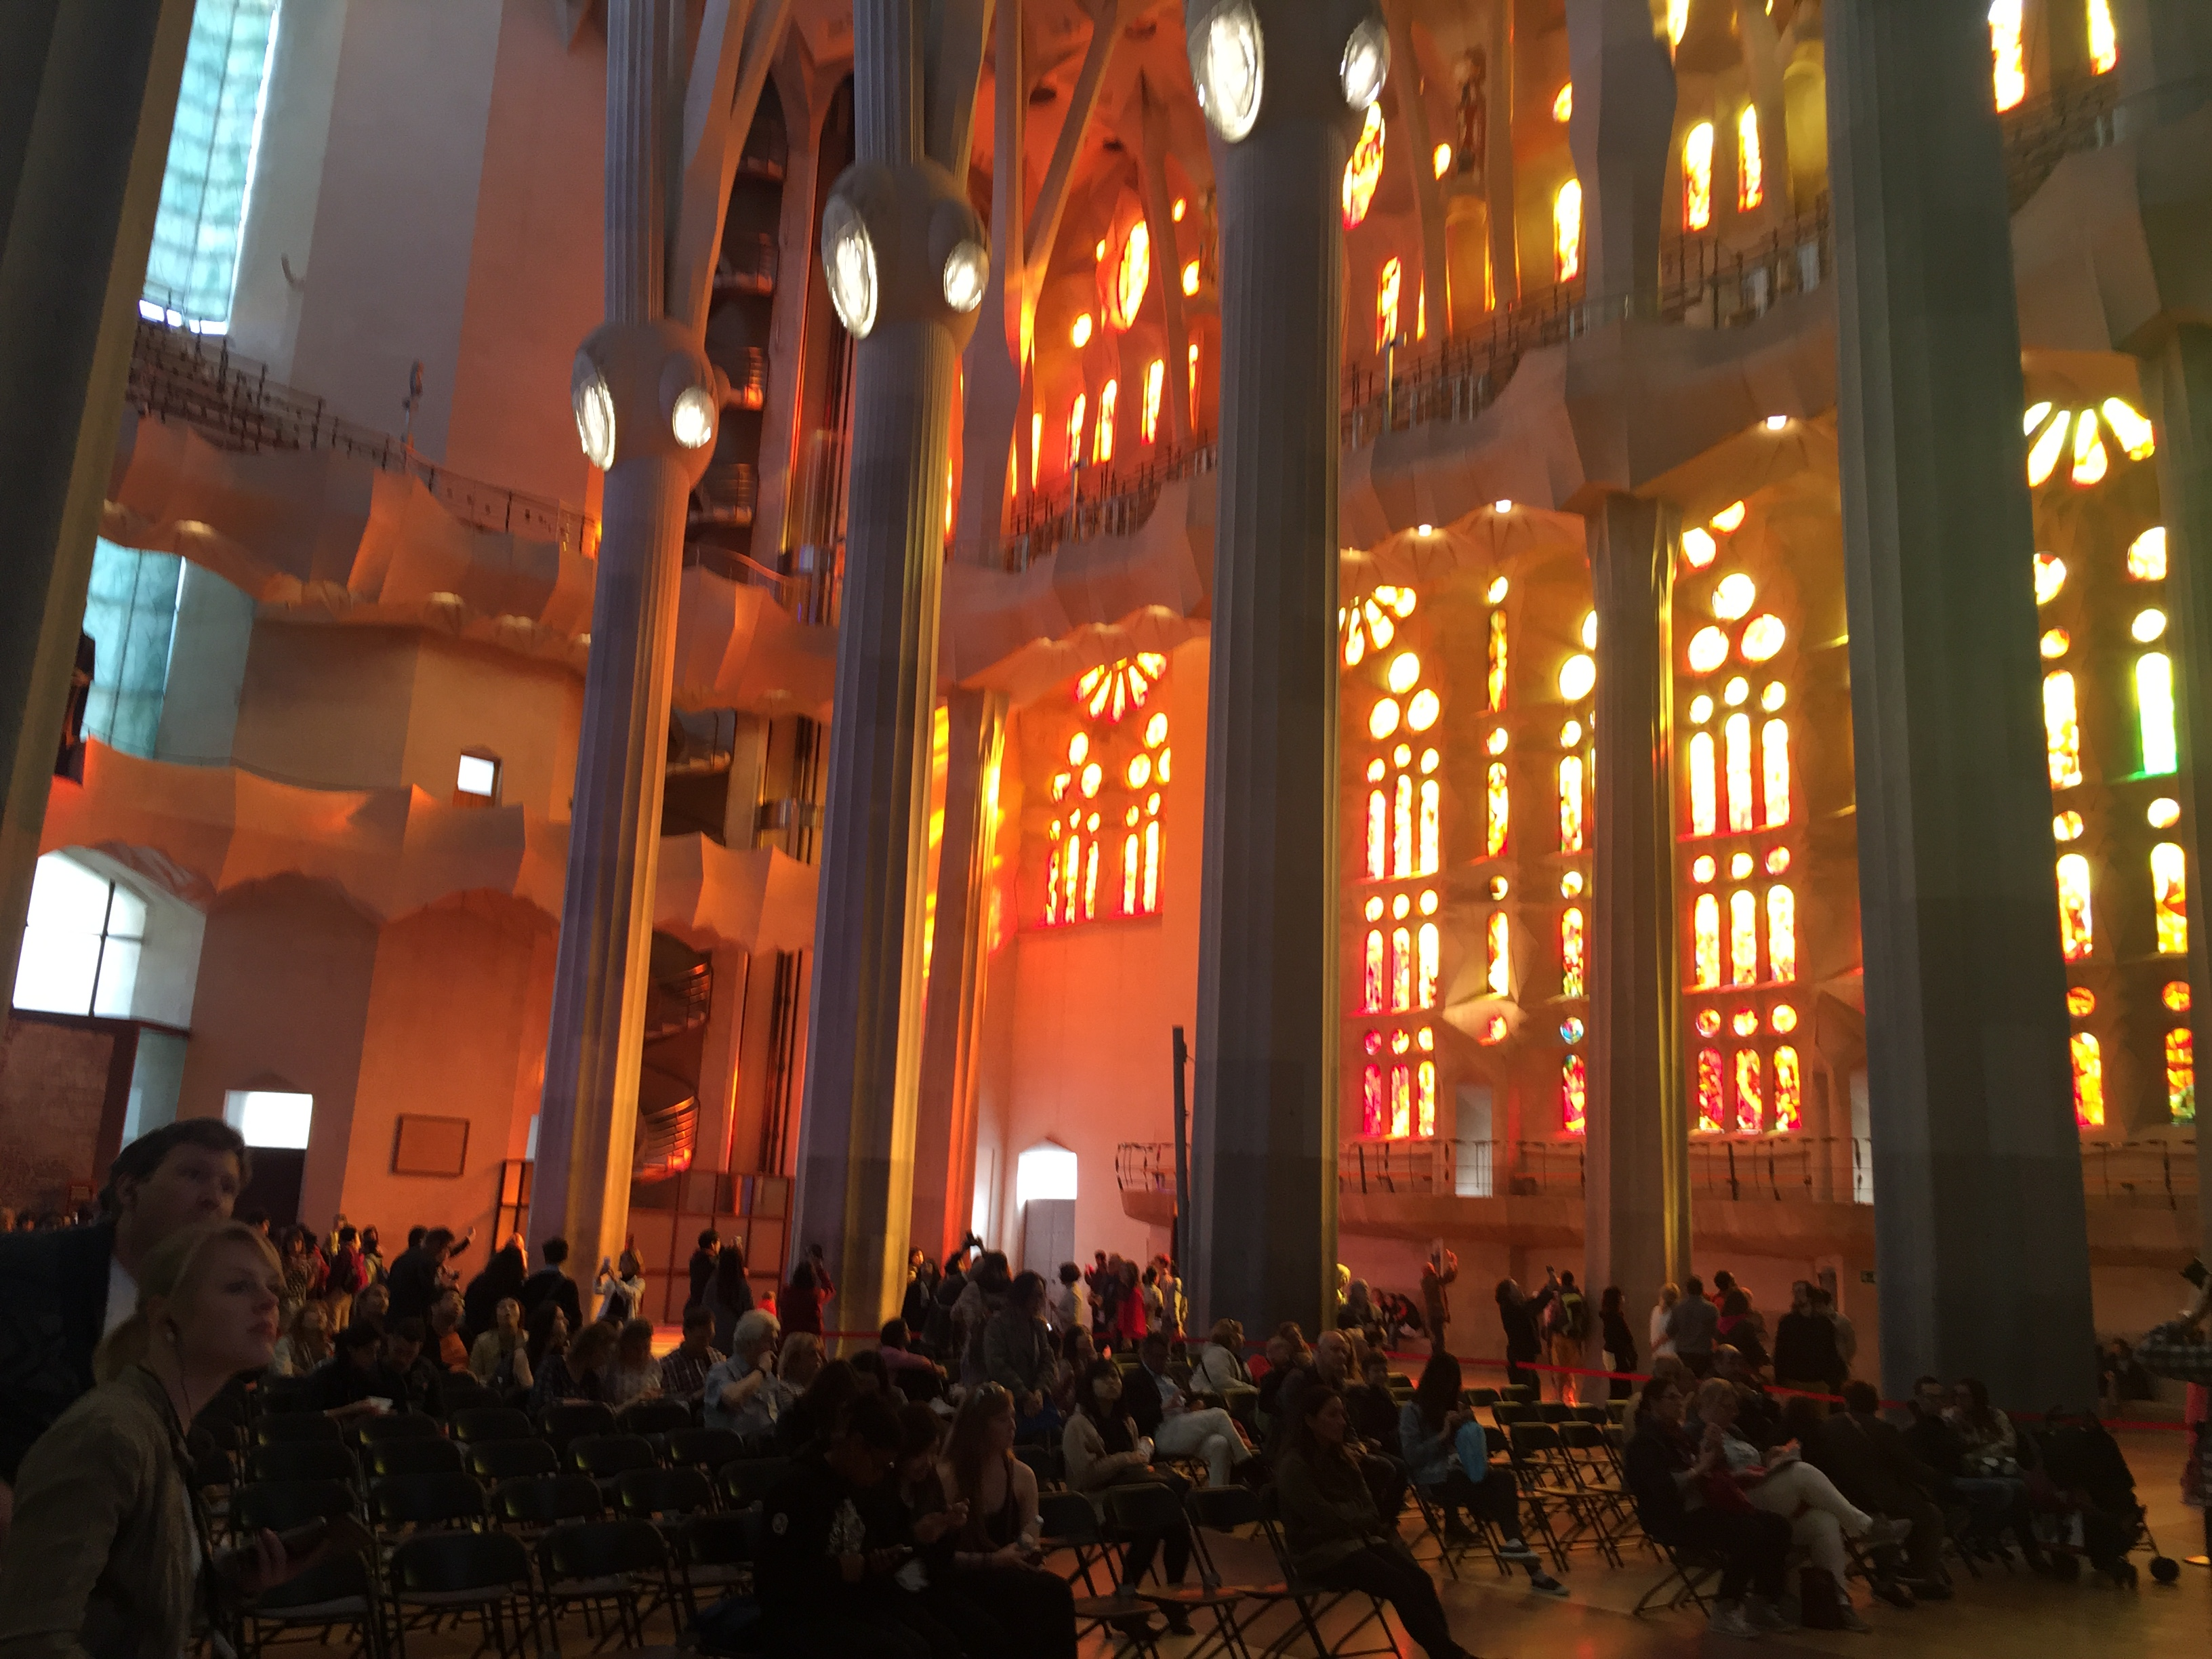
\includegraphics[width=.35\textwidth]{images/IMG_3268.JPG}};
		
		\node[inner sep=5pt] (graph1) at (0,-6)
		{
			\begin{tikzpicture}
			\node[draw, circle, fill=graphc2] (n1) at (0,-1) {};
			\node[draw, circle, fill=graphc3] (n2) at (1,-0.67) {};
			\node[draw, circle, fill=graphc4] (n3) at (2,-0.33) {};
			\node[draw, circle, fill=graphc2] (n4) at (0,-2) {};
			\node[draw, circle, fill=graphc3] (n5) at (1,-1.9) {};
			\node[draw, circle, fill=graphc4] (n6) at (2,-1.8) {};
			
			\draw[<->] (n1) -- (n2);
			\draw[<->] (n2) -- (n3);
			\draw[<->] (n1) -- (n4);
			\draw[<->] (n2) -- (n5);
			\draw[<->] (n4) -- (n5);
			\draw[<->] (n5) -- (n6);
			\end{tikzpicture}
		};
		
		\node[inner sep=5pt] (graph2) at (10,-6)
		{
			\begin{tikzpicture}
			\node[draw, circle] (n0) at (-1,-1.5) {};
			\node[draw, circle, fill=graphc1] (n7) at (-0.8,-0.33) {};
			\node[draw, circle, fill=graphc2] (n1) at (0,-1) {};
			\node[draw, circle, fill=graphc3] (n2) at (1,-0.67) {};
			\node[draw, circle, fill=graphc2] (n4) at (0,-2) {};
			\node[draw, circle, fill=graphc3] (n5) at (1,-1.9) {};
			
			\draw[<->] (n0) -- (n1);
			\draw[<->] (n0) -- (n4);
			\draw[<->] (n0) -- (n7);
			\draw[<->] (n1) -- (n2);
			\draw[<->] (n1) -- (n4);
			\draw[<->] (n2) -- (n5);
			\draw[<->] (n4) -- (n5);
			\end{tikzpicture}
		};
		
		\draw[->,thick] (sagrada1.east) -- (sagrada2.west)
		node[midway,fill=white] {Similarity};
		\draw[->,thick] (graph1.east) -- (graph2.west)
		node[midway,fill=white] {Similarity};
		
		\draw[->,thick] (sagrada1.south) -- (graph1.north)
		node[midway,fill=white] {Transform};
		\draw[->,thick] (sagrada2.south) -- (graph2.north)
		node[midway,fill=white] {Transform};
	\end{tikzpicture}
}
\caption{An example of the expected similarity between two views of the same scene. Similar objects and scenes should theoretically generate similar graphs after a suitable transformation, enabling recognition across images.\label{fig:intro-sim}}
\end{figure}

Graph models, long-explored in discrete mathematics, provide a simpler way of visualising problems.
Systems are broken down into \emph{vertices} and \emph{edges} between vertex pairs---capturing the relationships between objects or key features within a scene.
For many domains, this is an intuitive and effective representation, encoding rich semantics in a very natural way which enjoys use in computational chemistry \cite{Graph-Molecules-2,Graph-Molecules-3,Graph-Molecules-1}, biology \cite{Graph-Biology-1}, and graph database analysis.
Furthermore, exact graph search and similarity metrics (e.g.\ the \emph{subgraph isomorphism} and \emph{maximum common subgraph} problems, respectively) are well-understood and an area of continual research in the field of algorithms.
%?? part of idea---need effective models to know that our similarity algorithms are a good fit?

The main aim of this paper is to explore the hypothesis that, after suitable transformation, image similarity corresponds to graph similarity according to these known metrics; \cref{fig:intro-sim} gives a rough illustration of the concept.
In particular, this work focuses on character analysis and recognition, considering both the performance of graph models within a domain alongside the usefulness of any chosen analytic techniques.
By investigating these questions, this paper contributes:
\begin{itemize}
	\item A demonstration of the shortcomings of existing image graph work for generic matching (\Cref{sec:image-weakness}), by attempting similarity computation on graphs built using common techniques from the literature. %given that this also requires an investigation into the effectiveness of known graph similarity techniques, this motivates the development of new models.
	This weakness motivates the development of new modelling strategies.
	
%	\item Algorithms for decomposing textual images into a graph structured format, capturing elements of path curvature as the features for matching (\Cref{sec:algorithm}).
%	I demonstrate that the graph structure then allows the discovery of a supposed issue in the first algorithm, introducing path angle dynamics to make characters more distinct (\Cref{sec:algorithm:dual}).

	\item An algorithm for converting binary images into graphs, designed for use with images containing a clear path structure, such as character glyphs (\Cref{sec:algorithm}).
	Path curvature is the core feature for matching.
	
	\item A matching algorithm for these graphs, produced by modifying the $k\downarrow$ \cite{Between-MCS-SIP} procedure (\Cref{sec:k-down-mods}).
	This modified algorithm is used to compute graph similarity as part of a $k$-Nearest Neighbours classifier.
	
	\item An alternative graph model, capturing angle path dynamics using a ``dual graph''-like transformation (\Cref{sec:algorithm:dual}).
	This model arises in response to a perceived weakness in the first algorithm; this discovery is aided by the intuitive structure of the original graph model.
	
	\item An experimental evaluation of the matching accuracy of these models against datasets of handwritten and machine-generated character glyphs (\Cref{sec:evaluation}).

%	\item ?? Detail as paper written
\end{itemize}

%====================================================
\section{Graphs, Search and Similarity}
\label{sec:graph-search}
%====================================================

%?? Graph definitions etc
First, we must define graphs more precisely.
An undirected graph $\mathcal{G}$ may be written $\mathcal{G} = (V,E)$ for a vertex set $V$ and an edge set $E \subseteq \lbrace \lbrace u,v \rbrace : u,v \in V \rbrace $, i.e.\ each edge $e \in E$ is a set of two vertices from $V$.
To access these sets, I define the functions $\operatorname{V}(\mathcal{G})=V$ and $\operatorname{E}(\mathcal{G})=E$ to retrieve the vertex and edge set respectively.
For some $u,v \in V$, we may write $u \sim_\mathcal{G} v$ to mean $u$ and $v$ are adjacent vertices in $\mathcal{G}$ ($\lbrace u,v \rbrace \in E$), and use $N_\mathcal{G}(u)$ to refer to $u$'s \emph{neighbourhood}---the set of all vertices in $V \backslash \lbrace u \rbrace$ adjacent to $u$ in $\mathcal{G}$.
This definition allows loops, e.g.\ $u \sim_\mathcal{G} u$ with the caveat that $u \notin N_\mathcal{G}(u)$.
Additionally, the \emph{order} of $\mathcal{G}$ refers to the count of $\mathcal{G}$'s vertices ($\operatorname{Ord}(\mathcal{G})=|V|$), and the \emph{size} of $\mathcal{G}$ refers to the count of $\mathcal{G}$'s edges ($\operatorname{Sz}(\mathcal{G})=|E|$).
Where $\mathcal{G}$ is clear from context, the relevant subscripts will be elided.

The graphs produced by the techniques I outline are \emph{attributed undirected multigraphs}: vertices and edges may have labels, and each pair of vertices may share multiple edges.
Given domains $L_v, L_e$ for vertex and edge labels respectively, we redefine $\mathcal{G} = (V,E,\ell_v,\ell_e)$ for a vertex set $V$, an edge set $E$, a vertex label mapping $\ell_v: V \rightarrow L_v$ and an edge mapping $\ell_e: E \rightarrow \lbrace(\lbrace u,v \rbrace, l): u,v \in V, l \in L_e\rbrace$.
%For any vertex $v \in V$, its label in $\mathcal{G}$ is given as $l_\mathcal{G}(v)$.
We can succinctly describe the edges between any $u, v \in V$ with a sorted (non-decreasing) sequence of labels, $\operatorname{seq}_\mathcal{G}(u, v)$.
This allows us to define basic adjacency, and thus the basic neighbourhood: $u \sim_\mathcal{G} v \iff |\operatorname{seq}_\mathcal{G}(u,v)| \ge 1$.
For matching such graphs, we require three new neighbourhood definitions.
Given a sorted label sequence $s$, we may define the \emph{exact neighbourhood} $N^{=}_{s,\mathcal{G}}(u)$ as the set of all $v \in N_\mathcal{G}(u)$ such that $\operatorname{seq}_\mathcal{G}(u,v)=s$.
The \emph{sufficient neighbourhood} $N^{\succcurlyeq}_{s,\mathcal{G}}(u)$ is the set of all $v \in N_\mathcal{G}(u)$ where we may map each label in $s$ to a distinct label of equal value in $\operatorname{seq}_\mathcal{G}(u,v)$---we say that $s \preccurlyeq \operatorname{seq}_\mathcal{G}(u,v)$ if such a mapping exists.
Finally, the \emph{overlap neighbourhood} $N^{\circ}_{s,\mathcal{G}}(u)$ is the set of all $v \in N_\mathcal{G}(u)$ where at least one label in $s$ may be mapped to a label of equal value in $\operatorname{seq}_\mathcal{G}(u,v)$.
%=\lbrace v \in V \backslash \lbrace u \rbrace: \operatorname{seq}_\mathcal{G}(u,v)=s\rbrace$
For simplicity, I shall define the core search and similarity problems using undirected graphs.

Transformation from an image to a graph will create a graph whose structure corresponds to the image's content and invariants.
If an image $I$ contains an object, it is thus reasonable to assume that the graph produced from an image of only that object should be reproduced within $I$'s graph model---this may be useful when e.g., searching for a road sign in a view seen by an autonomous car.
This form of graph search is known as the \emph{subgraph isomorphism problem} (SIP), which is concerned with finding the exact structure of some pattern graph $\mathcal{P}=(V_\mathcal{P}, E_\mathcal{P})$ within a target graph $\mathcal{T}=(V_\mathcal{T}, E_\mathcal{T})$---an example is provided in \cref{fig:lit-sip}.
More precisely, for the non-induced variant of SIP the problem is to find an injective mapping $i : V_\mathcal{P} \rightarrow V_\mathcal{T}$ such that $\forall u,v \in V_\mathcal{P}, i(u) \neq i(v)$ and $u \sim_\mathcal{P} v \Rightarrow i(u) \sim_\mathcal{T} i(v)$, preserving adjacency and ensuring no two vertices of $\mathcal{P}$ are mapped to the same vertex of $\mathcal{T}$.
The induced variant additionally imposes that $\forall u,v \in V_\mathcal{P}, u \nsim_\mathcal{P} v \Rightarrow i(u) \nsim_\mathcal{T} i(v)$, ensuring that non-adjacent vertices in $\mathcal{P}$ must remain non-adjacent in the embedding in $\mathcal{T}$.
While SIP is \NP-Complete \cite{Cook-SAT-SIP-NP, Computers-and-Intractibility}, with modern algorithms such as \citeauthor{SIP-Glasgow}'s Glasgow solver it is computationally feasible for graphs on the order of several thousand vertices \cite{SIP-Glasgow}.
Trends in recent work have focused on increasing performance for larger instances through more costly filtering and pre-processing \cite{SIP-LAD, SIP-SND, SIP-Glasgow}---for this reason, older approaches such as VF2 \cite{SIP-VF2} remain competitive on smaller instances \cite{SIP-Hard-Instances}.
%The constraint programming 
%?? SIP \cite{SIP-VF2, SIP-LAD, SIP-SND, SIP-Glasgow}, Regin filtering \cite{AllDiff}, Complexity \cite{Cook-SAT-SIP-NP}

\begin{figure}
	\centering
	\resizebox{\columnwidth}{!}{
	\begin{tikzpicture}
	
	\node[label=below:{$\mathcal{P}$}] (p) at (0,0){
		\begin{tikzpicture}[scale=1]
		\begin{scope}[auto, every node/.style={draw,circle,minimum size=2em,inner sep=1},node distance=2cm]
		\node[draw, circle] (n1) at (0,0) {a};
		\node[draw, circle] (n2) at (0,-1) {c};
		\node[draw, circle] (n3) at (1,0) {b};
		\node[draw, circle] (n4) at (1,-1) {d};
		\end{scope}
		
		\draw[-] (n1) -- (n3);
		\draw[-] (n2) -- (n4);
		\draw[-] (n1) -- (n4);
		\draw[-] (n2) -- (n3);
		\draw[-] (n3) -- (n4);
		\end{tikzpicture}
	};
	
	\node[label=below:{$\mathcal{T}$}] (t) at (4,0){
		\begin{tikzpicture}[scale=1]
		\begin{scope}[auto, every node/.style={draw,circle,minimum size=2em,inner sep=1},node distance=2cm]
		\node[draw, circle] (n1) at (2,0) {2};
		\node[draw, circle] (n2) at (0,-1) {4};
		\node[draw, circle] (n3) at (1,0) {1};
		\node[draw, circle] (n4) at (1,-1) {5};
		
		\node[draw, circle] (n5) at (2,-1) {6};
		\node[draw, circle] (n6) at (3,0) {3};
		\end{scope}
		
		\draw[-] (n1) -- (n3);
		\draw[-] (n2) -- (n4);
		\draw[-] (n1) -- (n4);
		\draw[-] (n2) -- (n3);
		\draw[-] (n3) -- (n4);
		
		\draw[-] (n5) -- (n6);
		\draw[-] (n1) -- (n6);
		\draw[-] (n3) -- (n5);
		\end{tikzpicture}
	};
	
	\node[label=below:{Embedding}] (em) at (9,0){
		\begin{tikzpicture}[scale=1]
		\begin{scope}[auto, every node/.style={draw,circle,minimum size=2em,inner sep=1},node distance=2cm]
		\node[draw, circle, fill=uofgpumpkin] (n1) at (2,0) {2};
		\node[draw, circle, fill=uofgpumpkin] (n2) at (0,-1) {4};
		\node[draw, circle, fill=uofgpumpkin] (n3) at (1,0) {1};
		\node[draw, circle, fill=uofgpumpkin] (n4) at (1,-1) {5};
		
		\node[draw, circle] (n5) at (2,-1) {6};
		\node[draw, circle] (n6) at (3,0) {3};
		\end{scope}
		
		\draw[-, color=uofgpumpkin] (n1) -- (n3);
		\draw[-, color=uofgpumpkin] (n2) -- (n4);
		\draw[-, color=uofgpumpkin] (n1) -- (n4);
		\draw[-, color=uofgpumpkin] (n2) -- (n3);
		\draw[-, color=uofgpumpkin] (n3) -- (n4);
		
		\draw[-] (n5) -- (n6);
		\draw[-] (n1) -- (n6);
		\draw[-] (n3) -- (n5);
		\end{tikzpicture}
	};
	
	\draw[->, thick] (t) -- (em);
	
\end{tikzpicture}
}
\caption{
		An example of the subgraph isomorphism problem between two graphs $\mathcal{P}$ and $\mathcal{T}$.
		$\mathcal{P}$'s embedding within $\mathcal{T}$ is highlighted in orange---this is a valid matching in both the induced and non-induced SIP variants.
		\label{fig:lit-sip}
}
\end{figure}

%?? MCS \cite{Between-MCS-SIP}, James+Ciaran+Pat's new paper too \cite{MCS-McSplit}, complexity \cite[p.\ 74--75]{Computers-and-Intractibility}
In reality, elements of an object's graph structure may not be reproduced in the graph of an embedding due to either occlusion, image distortion or object scale.
In this case, it is worthwhile to examine how much two image graphs have in common to identify common elements and substructures.
Between two graphs $\mathcal{P}$ and $\mathcal{T}$ this is known as the \emph{maximum common subgraph problem} (MCS), which is the search for the largest subgraph of $\mathcal{P}$ which is isomorphic to some subgraph of $\mathcal{T}$ as in SIP.
\Cref{fig:lit-mcs} offers an example instance.
While this problem as described is \NP-Hard, it is considerably harder in practice than SIP---the current state-of-the-art, McSplit, can operate on graphs of order 35--40 \cite{MCS-McSplit}, where other approaches are limited to around 30 vertices.
Even so, this approach applies only to the induced variant of MCS and largely prevents the addition of side constraints.
For such flexibility we must consider either $k\downarrow$ \cite{Between-MCS-SIP}, a repeated application of the Glasgow SIP solver excluding $k$ vertices, or a max-clique-based approach using the \emph{association graph encoding} \cite{MCS-Clique-CP}.
In this regard there is a trade-off to be made: while the clique-based approach still achieves the best performance on labelled instances \cite{MCS-McSplit}, $k\downarrow$ requires far less memory to process high-order graphs.
I choose to examine and modify $k\downarrow$ for these reasons, but this still requires that the order of any graphs must remain small to perform occlusion-robust matching with this technique.

By computing similar structures between any two graphs as above, we may then quantify how similar they are by considering the order of the MCS.
This is in turn a key part of establishing how \emph{dissimilar} a pair of graphs are, and given that MCS order does not take into account the sizes of $\mathcal{P}$ or $\mathcal{T}$ such a metric is more desirable for global classification.
We may then use the MCS to compute the number of discrete changes needed to transform $\mathcal{P}$ into $\mathcal{T}$---the \emph{graph edit distance} (GED) \cite{GraphEditDist-MCS}.
For classification purposes, I consider a simplified expression which disregards edge costs:
$$ \operatorname{GED}(\mathcal{P}, \mathcal{T}) = \operatorname{Ord}(\mathcal{P}) + \operatorname{Ord}(\mathcal{T}) - 2 \operatorname{Ord}(\operatorname{MCS}(\mathcal{P}, \mathcal{T})) $$

\begin{figure}
	\centering
	\resizebox{0.8\columnwidth}{!}{
	\begin{tikzpicture}
	
	\node[label=below:{$\mathcal{P}$}] (p) at (0,0){
		\begin{tikzpicture}[scale=1]
		\begin{scope}[auto, every node/.style={minimum size=2em,inner sep=1},node distance=2cm]
		\node[draw, circle] (n1) at (0,0) {a};
		\node[draw, circle] (n2) at (0,-1) {c};
		\node[draw, circle] (n3) at (1,0) {b};
		\node[draw, circle] (n4) at (1,-1) {d};
		
		\draw[-] (n1) -- (n3);
		\draw[-] (n2) -- (n4);
		\draw[-] (n1) -- (n4);
		\draw[-] (n2) -- (n3);
		\draw[-] (n3) -- (n4);
		\end{scope}
		\end{tikzpicture}
	};
	
	\node[label=below:{$\mathcal{T}$}] (t) at (3,0){
		\begin{tikzpicture}[scale=1]
		\begin{scope}[auto, every node/.style={draw,circle,minimum size=2em,inner sep=1},node distance=2cm]
		\node[draw, circle] (n1) at (0,0) {1};
		\node[draw, circle] (n2) at (0,-1) {3};
		\node[draw, circle] (n3) at (1,0) {2};
		\node[draw, circle] (n4) at (1,-1) {4};
		\end{scope}
		
		\draw[-] (n1) -- (n3);
		\draw[-] (n2) -- (n4);
		\draw[-] (n1) -- (n2);
		\draw[-] (n2) -- (n3);
		\draw[-] (n3) -- (n4);
		
		\end{tikzpicture}
	};
	
	\node[label=below:{Embedding}] (em) at (7,0){
		\begin{tikzpicture}[scale=1]
		\begin{scope}[auto, every node/.style={draw,circle,minimum size=2em,inner sep=1},node distance=2cm]
		\node[draw, circle] (n1) at (0,0) {a};
		\node[draw, circle, fill=uofgpumpkin] (n2) at (0,-1) {c};
		\node[draw, circle, fill=uofgpumpkin] (n3) at (1,0) {b};
		\node[draw, circle, fill=uofgpumpkin] (n4) at (1,-1) {d};
		
		\draw[-] (n1) -- (n3);
		\draw[-, color=uofgpumpkin] (n2) -- (n4);
		\draw[-] (n1) -- (n4);
		\draw[-, color=uofgpumpkin] (n2) -- (n3);
		\draw[-, color=uofgpumpkin] (n3) -- (n4);
		
		\node[draw, circle] (n1') at (2,0) {1};
		\node[draw, circle, fill=uofgpumpkin] (n2') at (2,-1) {3};
		\node[draw, circle, fill=uofgpumpkin] (n3') at (3,0) {2};
		\node[draw, circle, fill=uofgpumpkin] (n4') at (3,-1) {4};
		
		
		\draw[-] (n1') -- (n3');
		\draw[-, color=uofgpumpkin] (n2') -- (n4');
		\draw[-] (n1') -- (n2');
		\draw[-, color=uofgpumpkin] (n2') -- (n3');
		\draw[-, color=uofgpumpkin] (n3') -- (n4');
		\end{scope}
		\end{tikzpicture}
	};
	
	\draw[->, thick] (t) -- (em);
	
\end{tikzpicture}
}
\caption{
		An example of the maximum common subgraph problem between two graphs $\mathcal{P}$ and $\mathcal{T}$.
		The MCS's embedding within both $\mathcal{P}$ and $\mathcal{T}$ is highlighted in orange.
		Note that this embedding is not unique, although for this choice of $\mathcal{P}$ and $\mathcal{T}$ the MCS itself is.
		\label{fig:lit-mcs}
}
\end{figure}

%====================================================
\section{On Existing Image Graph Models}
\label{sec:image-weakness}
%====================================================

%\citeauthor{Plane-Graphs-From-Images} \cite{Plane-Graphs-From-Images}

%?? Approaches such as seen in \cite{Submap-Iso-Images} use Delaunay -- Enhanced by structural cues such as in \cite{Plane-Graphs-From-Images}

\begin{figure*}
	\centering
	\begin{subfigure}[b]{0.22\textwidth}
		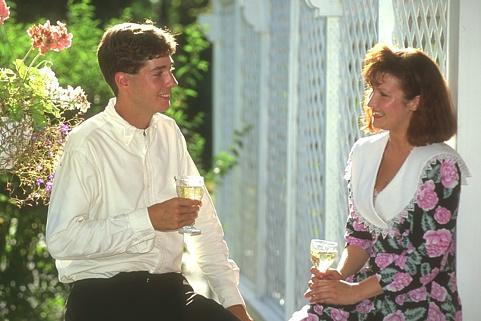
\includegraphics[width=\textwidth]{images/bsd-157055}
		\caption{BSD test image}
		\label{fig:explor-bsd}
	\end{subfigure}
	~
	\begin{subfigure}[b]{0.35\textwidth}
		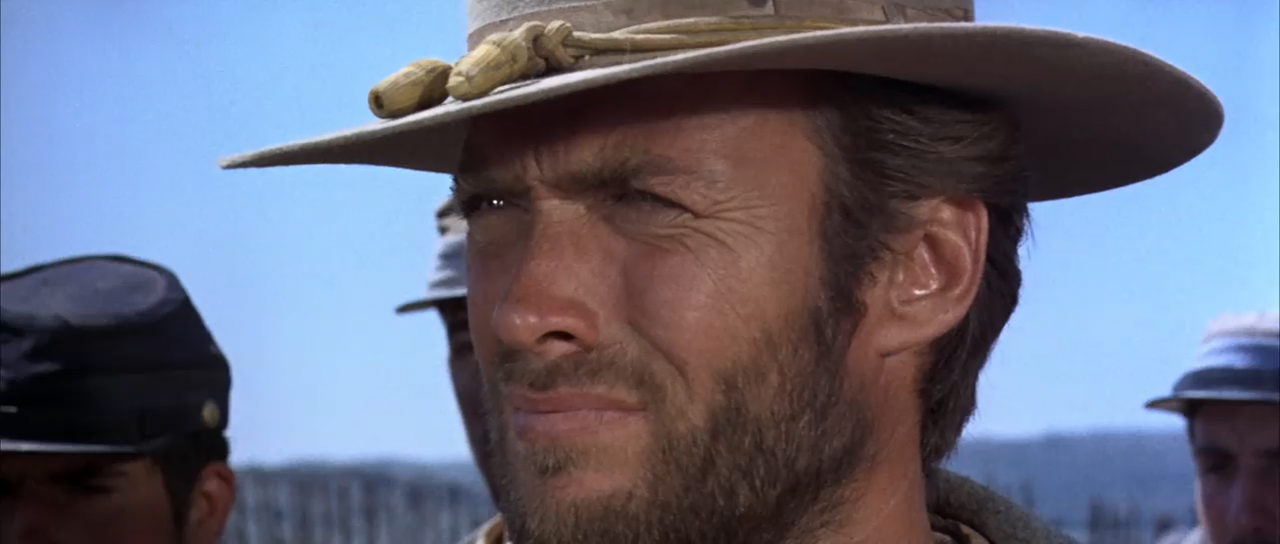
\includegraphics[width=\textwidth]{images/gbu2}
		\caption{Film frame 1}
		\label{fig:explor-ff1}
	\end{subfigure}
	~
	\begin{subfigure}[b]{0.35\textwidth}
		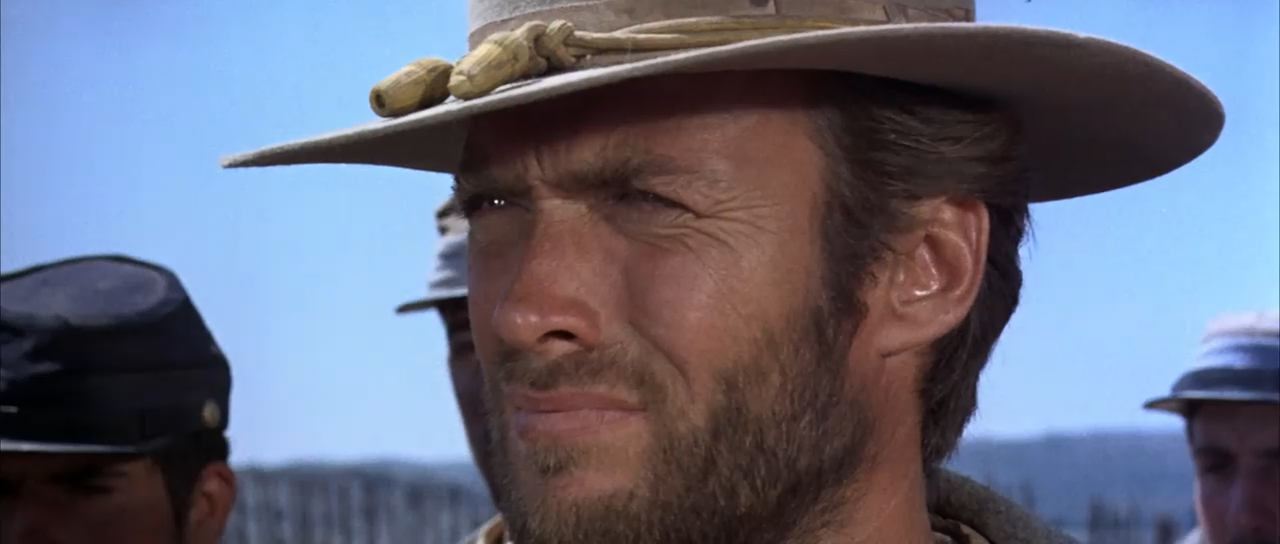
\includegraphics[width=\textwidth]{images/gbu3}
		\caption{Film frame 2}
		\label{fig:explor-ff2}
	\end{subfigure}
	
	\vspace{0.5em}
	
	\caption{
		Images used for evaluation of \citeauthor{Plane-Graphs-From-Images}'s \cite{Plane-Graphs-From-Images} approach.
	}
\end{figure*}

\begin{figure*}
	\centering
	\begin{subfigure}[b]{0.22\textwidth}
		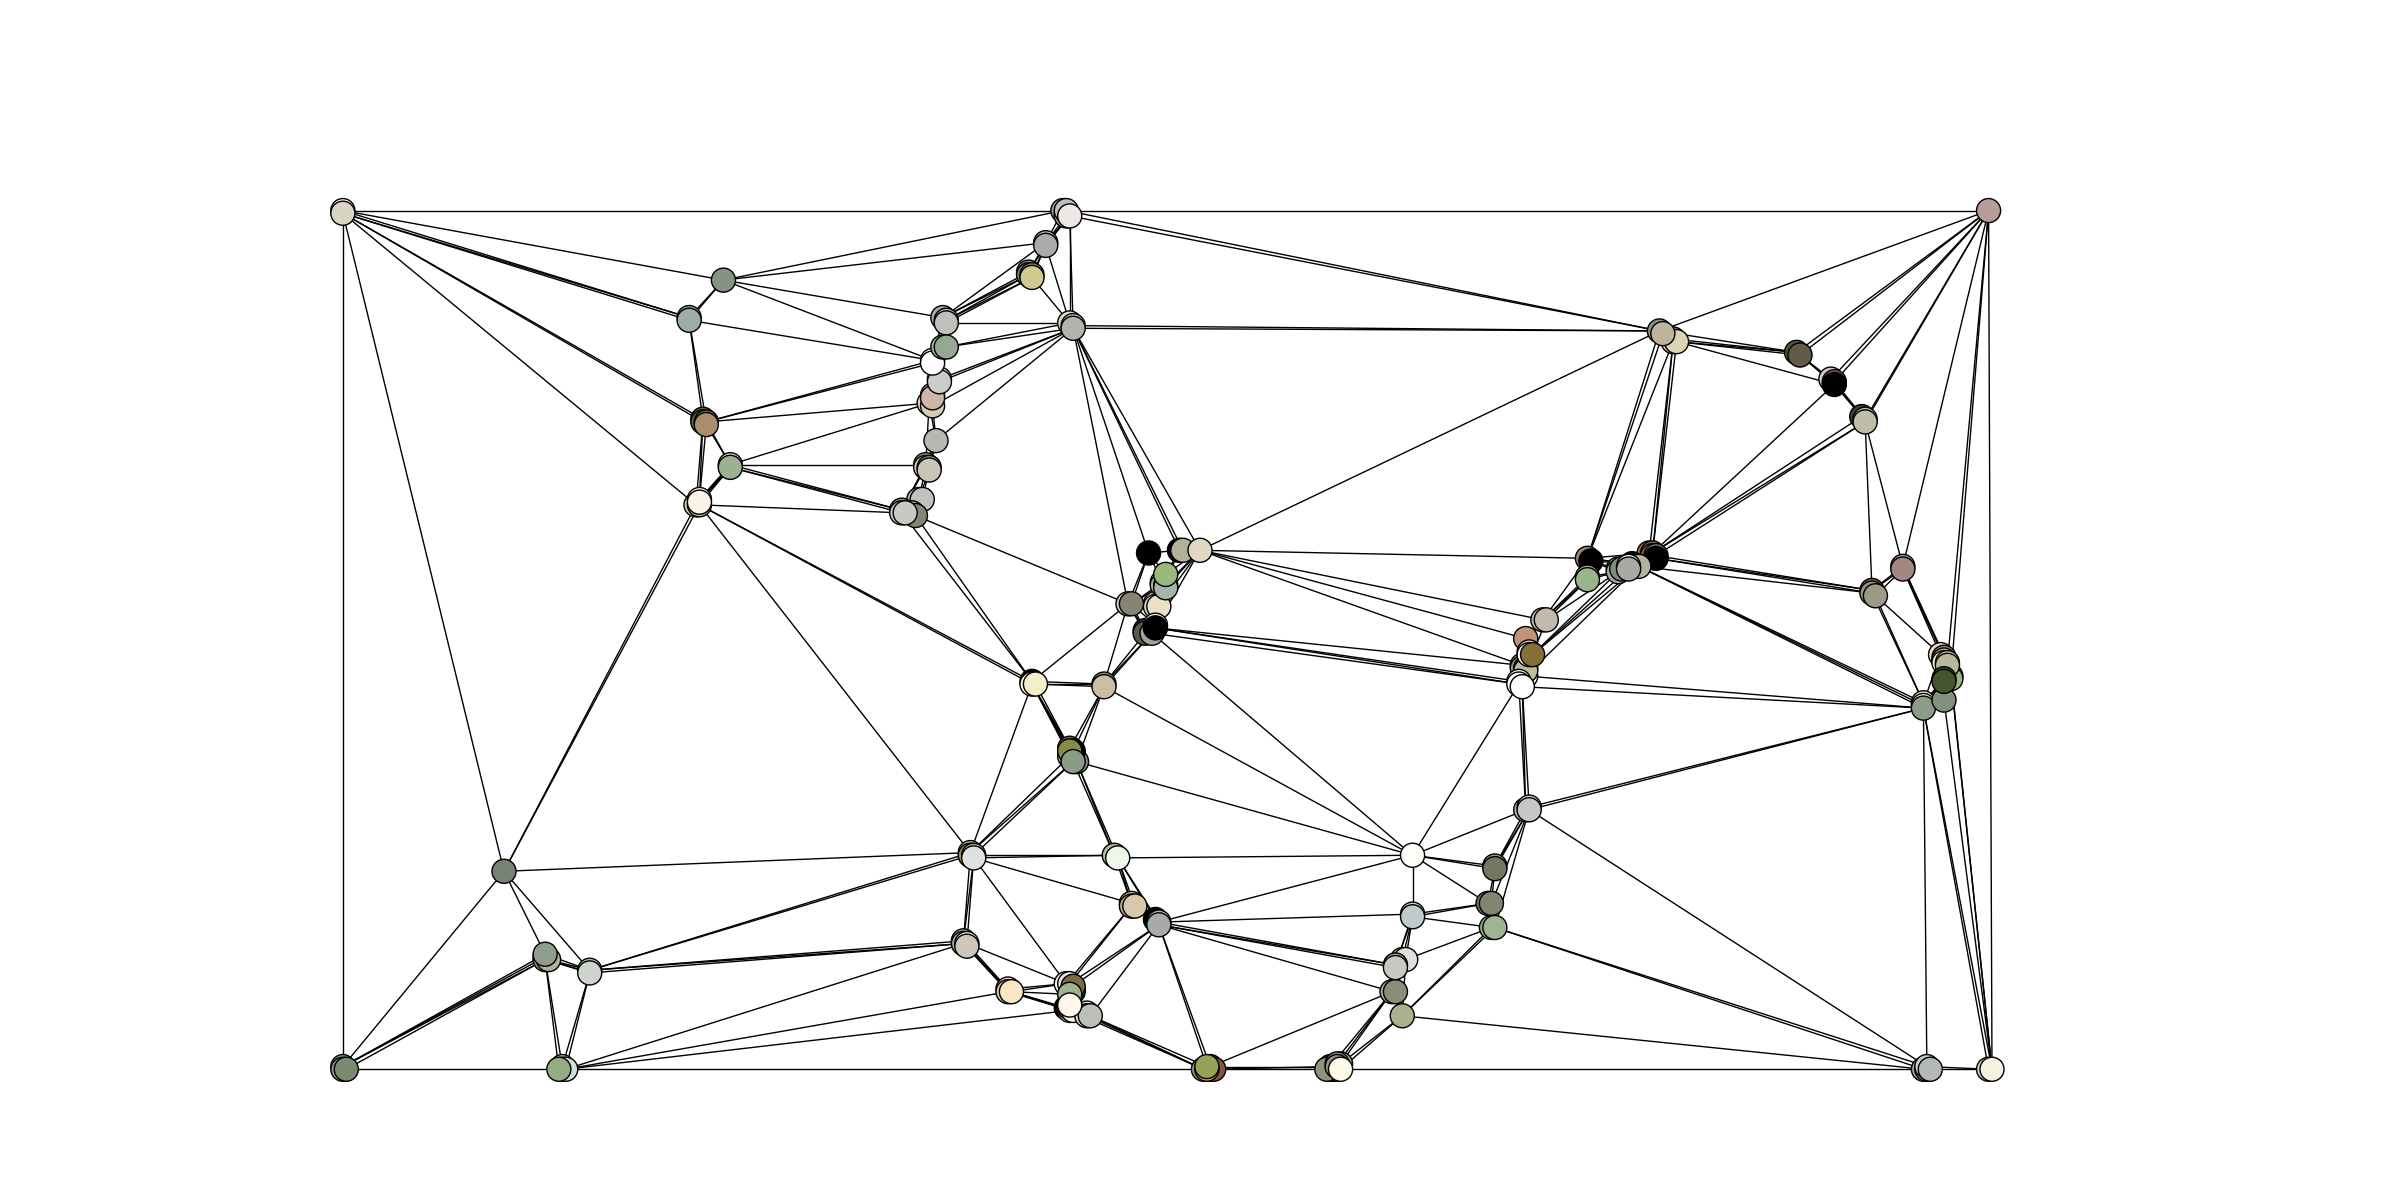
\includegraphics[width=\textwidth]{img-results/nrm}
		\caption{
				BSD test image, normal.
				$|V|=245$, $|E|=707$.
		}
		\label{fig:explor-bsdnrmgraph}
	\end{subfigure}
	~
	\begin{subfigure}[b]{0.22\textwidth}
		
\includegraphics[width=\textwidth]{img-results/180}
		\caption{
				BSD test image, \SI{180}{\degree} rotation.
				$|V|=247$, $|E|=705$.
		}
		\label{fig:explor-bsd180graph}
	\end{subfigure}
	~
	\begin{subfigure}[b]{0.22\textwidth}
		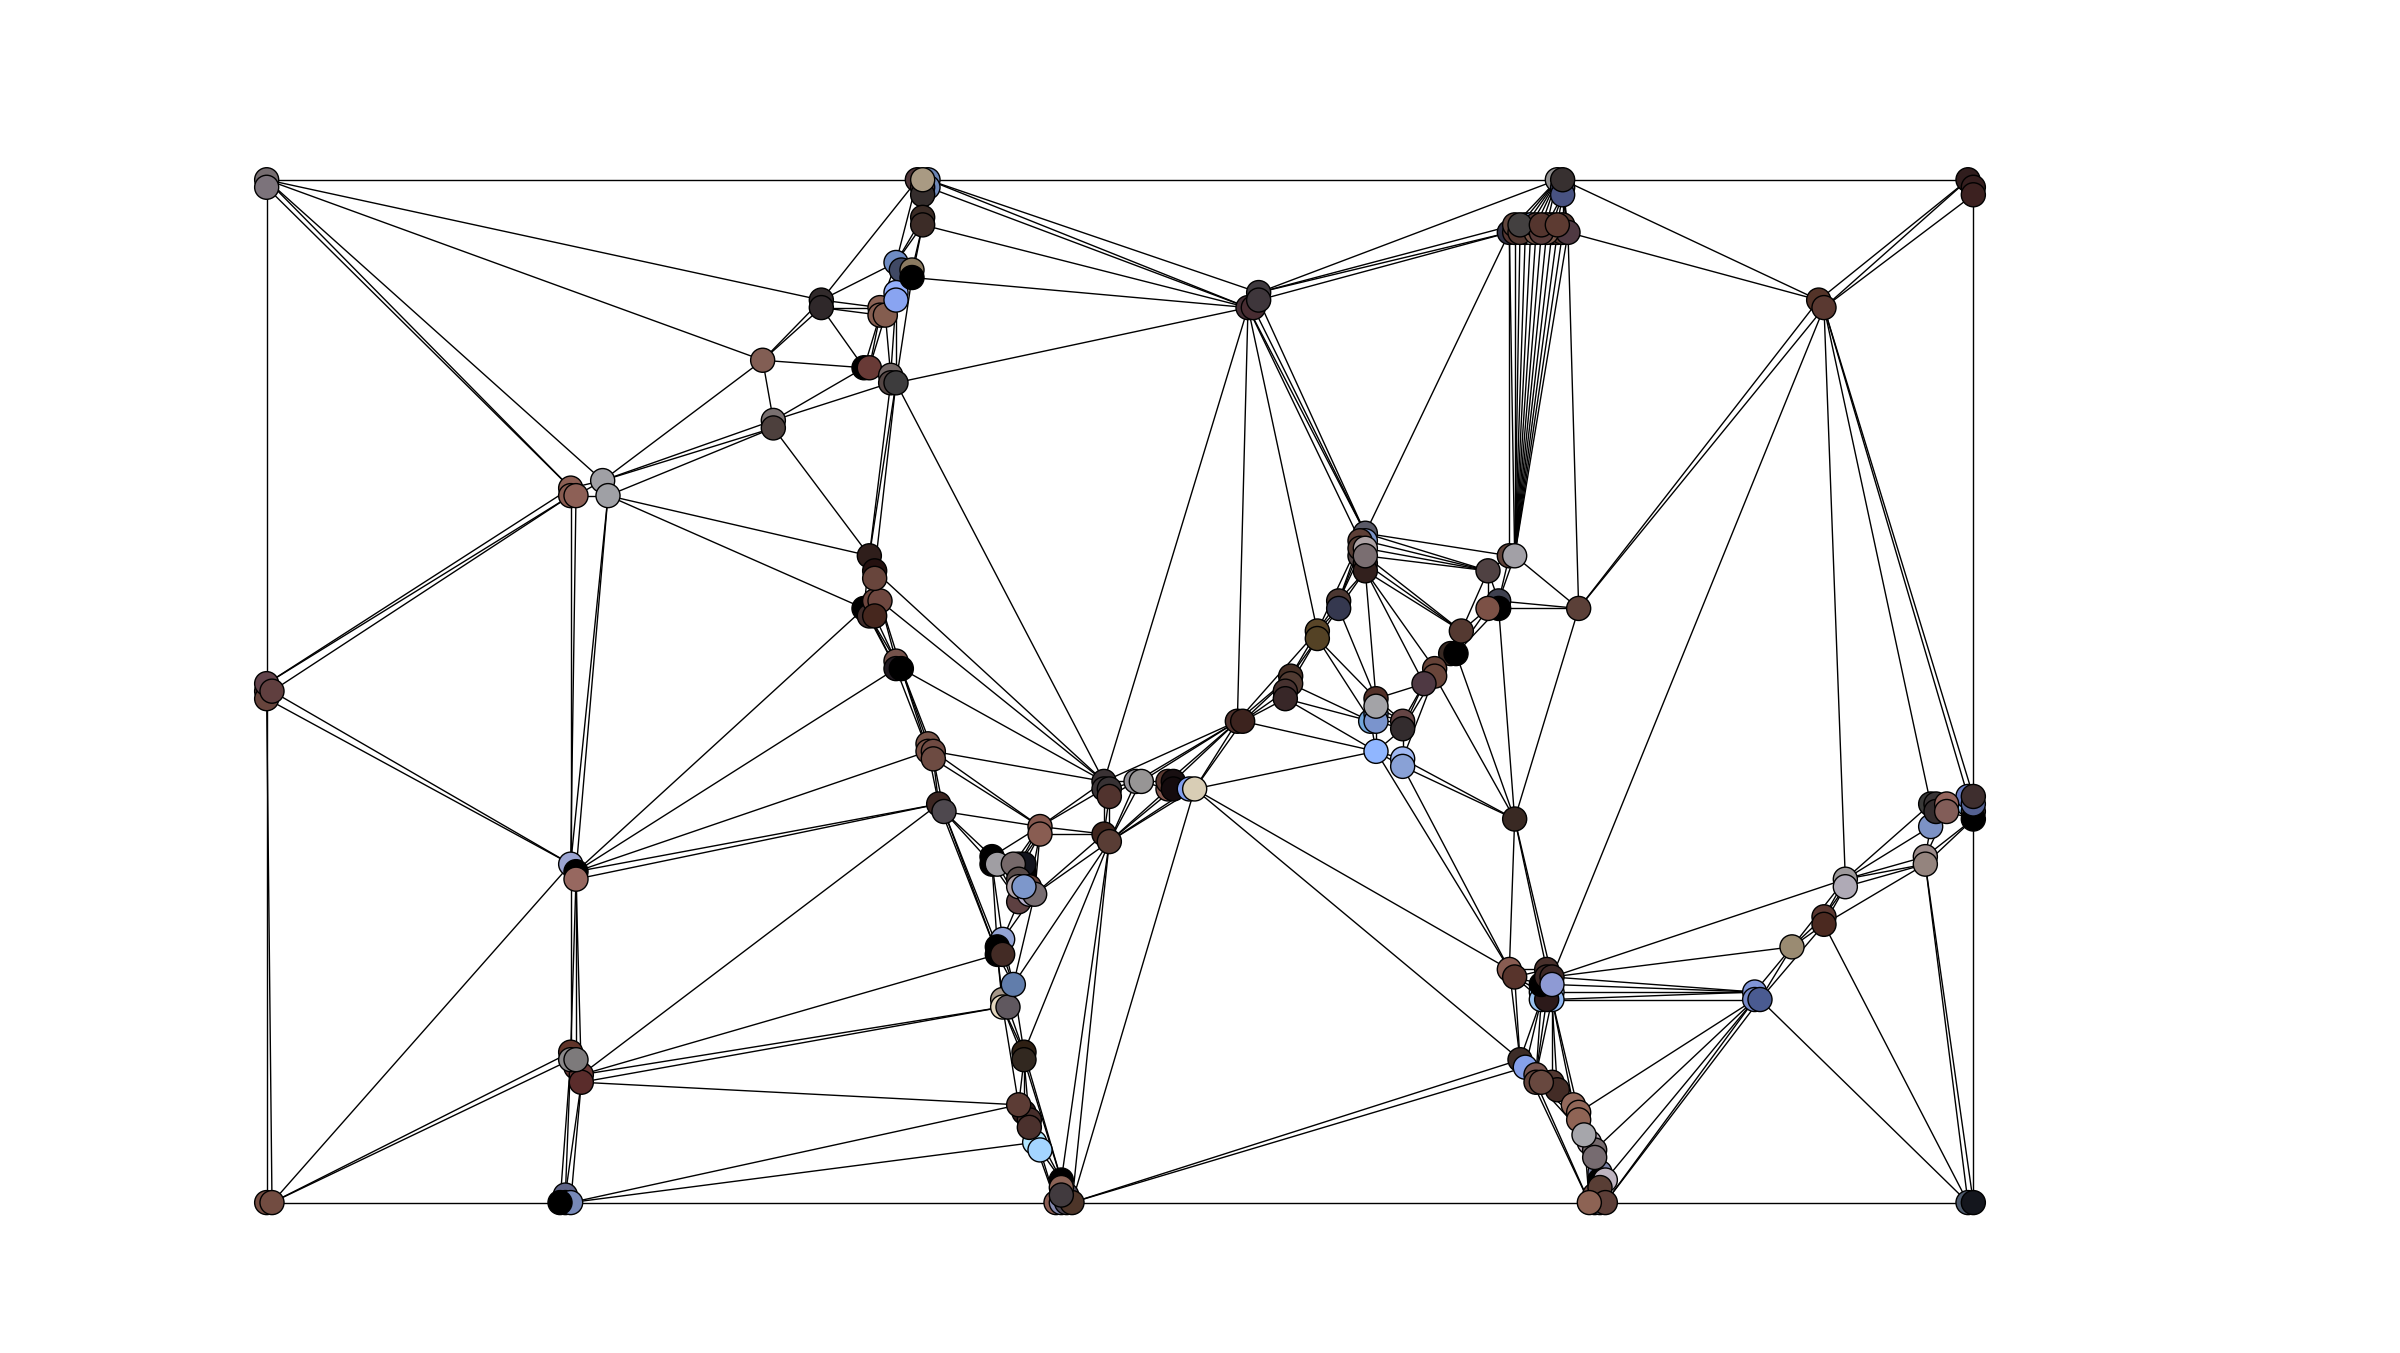
\includegraphics[width=\textwidth]{img-results/gbu-smr2-graph}
		\caption{
				Film frame 1.
				$|V|=264$, $|E|=755$.
		}
		\label{fig:explor-ff1graph}
	\end{subfigure}
	~
	\begin{subfigure}[b]{0.22\textwidth}
		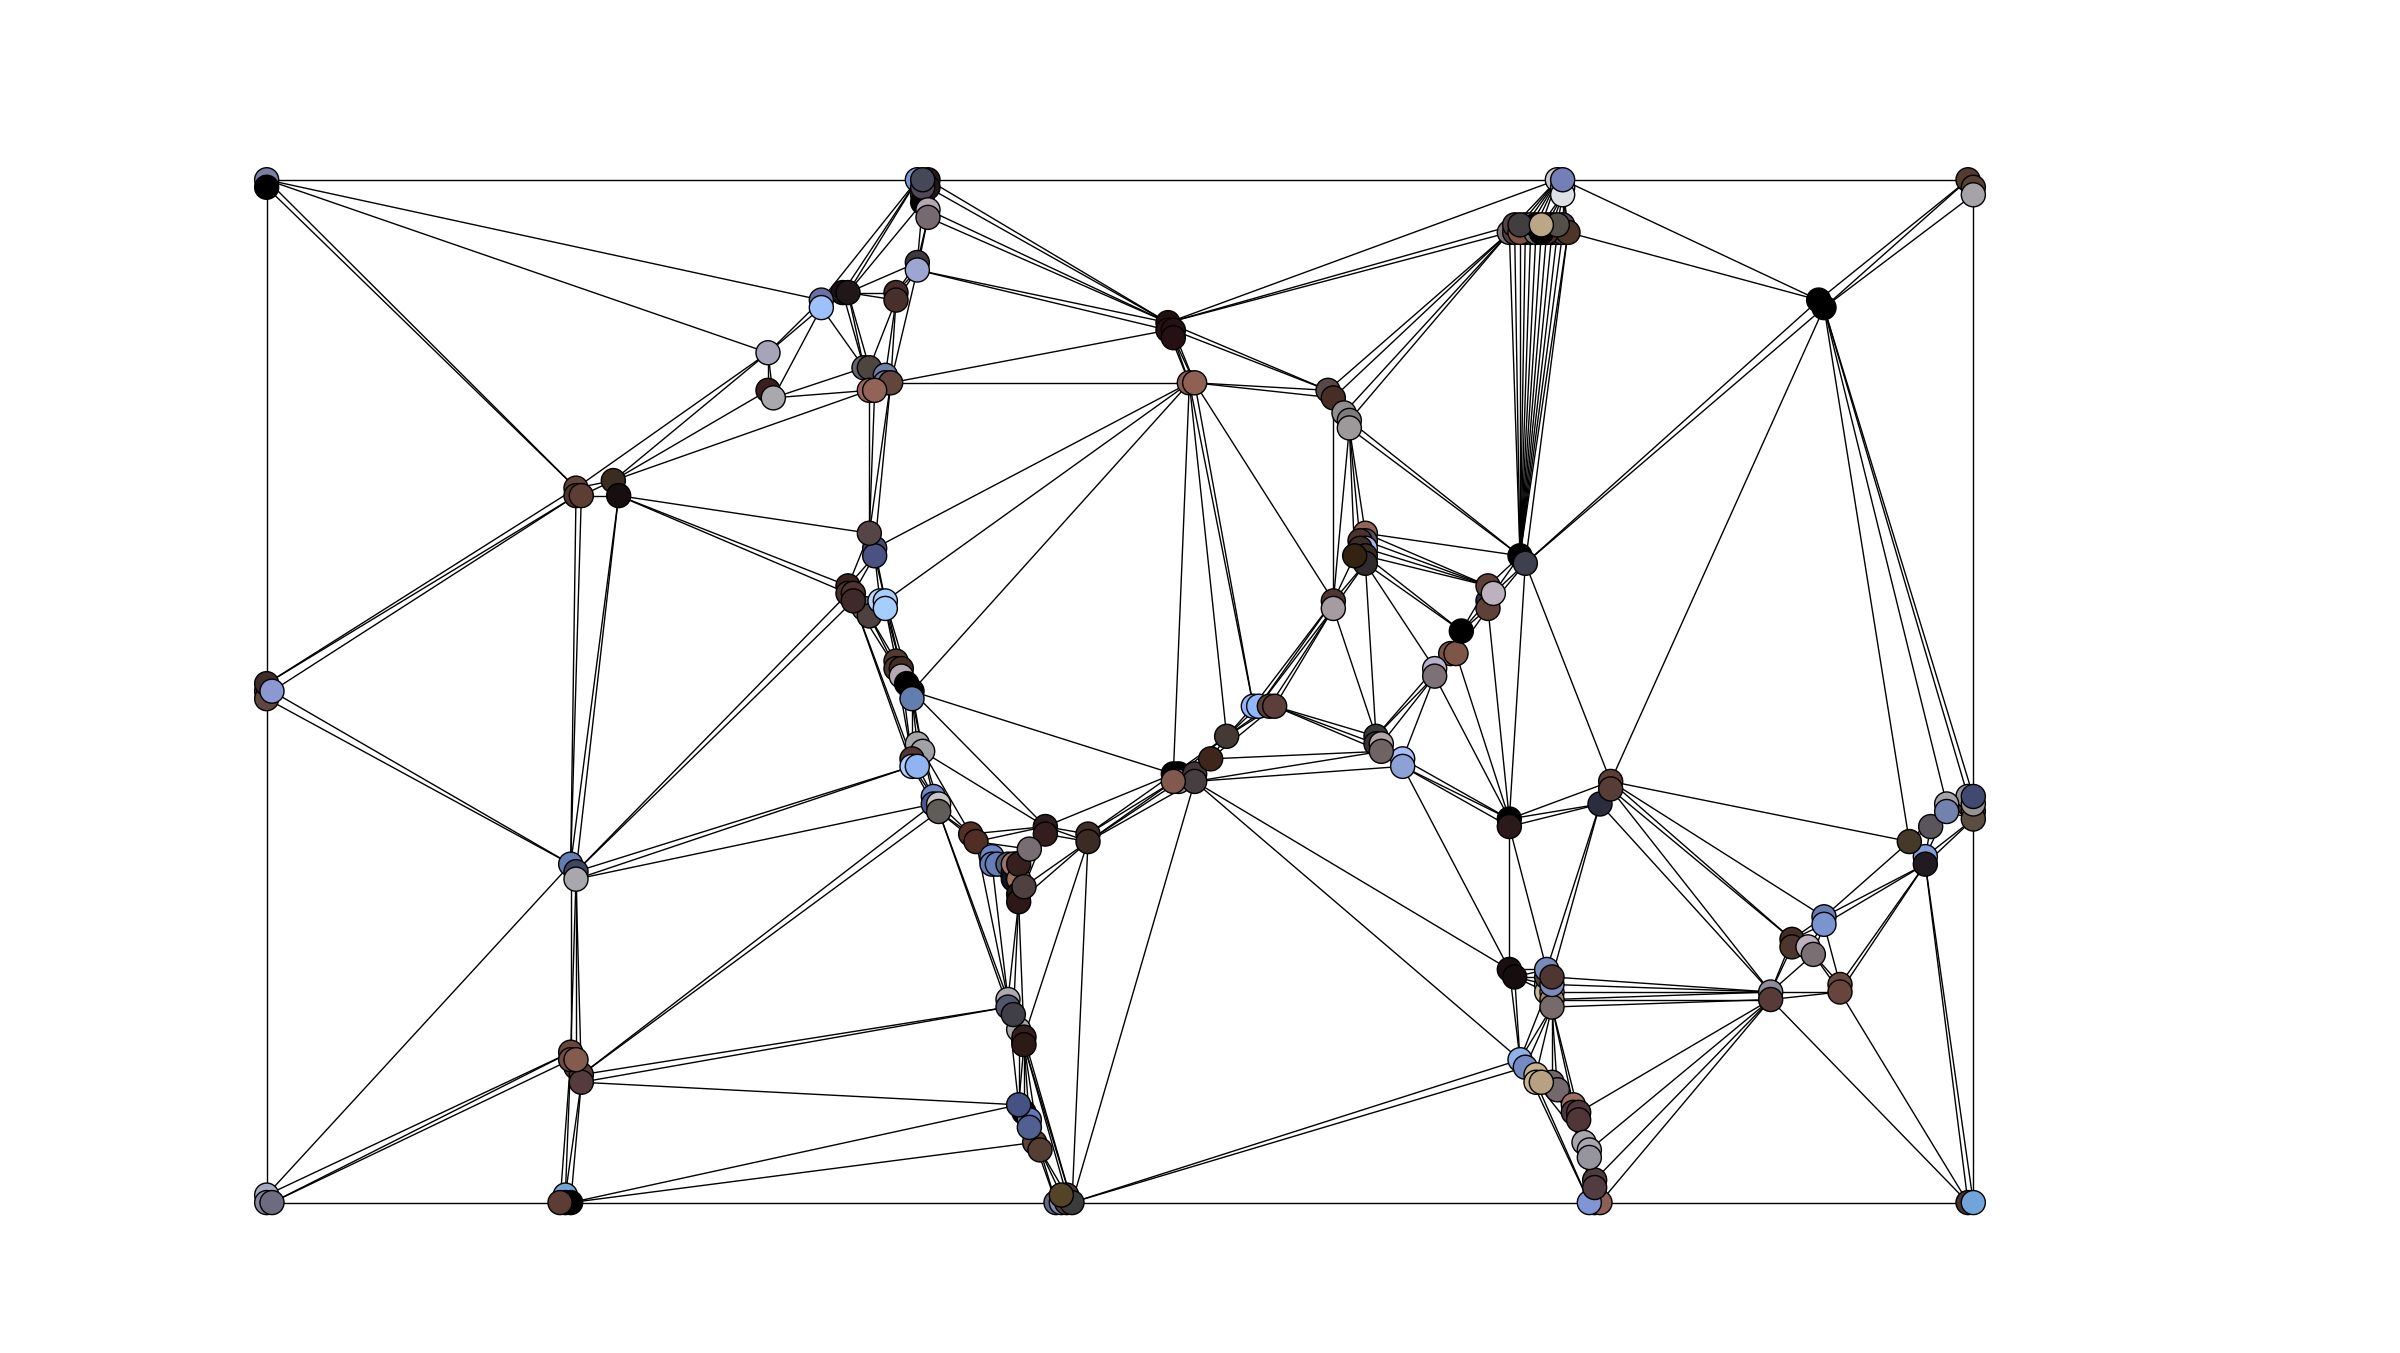
\includegraphics[width=\textwidth]{img-results/gbu-smr3-graph}
		\caption{
				Film frame 2.
				$|V|=260$, $|E|=743$.
		}
		\label{fig:explor-ff2graph}
	\end{subfigure}
	
	\vspace{0.5em}
	
	\caption{
		Graph output after boundary walking and Delaunay triangulation.
		$|V|$ and $|E|$ denote the vertex count and edge count, respectively.
	}
\end{figure*}

For graph modelling of generic images, present techniques typically build graphs by applying the \emph{Delaunay triangulation} \cite{Delaunay} to a set of interest pixels located within an image.
This process places edges between vertices with coordinate labels to construct a face-connected plane graph; specifically, where each face is a triangle.
Crucially, this mesh is subject to one key criterion designed to minimise the incidence of sliver triangles: no point may lie inside the circumcircle of any produced triangle.
Efficient algorithms exist for its computation \cite{DelaunayAlgs,DelaunayModern}.
This avenue is explored briefly by \citeauthor{Submap-Iso-Images} \cite{Submap-Iso-Images}, and expanded upon by \citeauthor{Plane-Graphs-From-Images} to make use of structural cues provided by image segmentation algorithms \cite{Plane-Graphs-From-Images}.
The authors of these approaches assess the effectiveness of their models by either searching for an image cropping within itself (using \emph{submap} isomorphism) or by quantifying the ``loss'' incurred by reconstruction from the generated graph.
In this regard much is made of matching of graphs \emph{within} an image, and not \emph{between} images; making it unclear whether any discriminative features are captured or modelled in a way that allows matching using MCS algorithms.

%?? Use existing work from proposal as basis
%?? No capture of discriminative features
To investigate this, I implemented \citeauthor{Plane-Graphs-From-Images}'s algorithm in Python, using \textit{scikit-image}\footnote{\url{http://scikit-image.org/}} functions for segmentation and interest pixel detection.
Two experiments were performed:
\begin{enumerate}
	\item Establishing whether graphs of a test image from the Berkeley Segmentation Dataset \cite{BerkeleyDatabase} (\cref{fig:explor-bsd}) before and after \SI{180}{\degree} rotation were isomorphic, and measuring their similarity if not.
	\item Measuring the similarity between two adjacent frames of Sergio Leone's \emph{The Good, the Bad and the Ugly} (\cref{fig:explor-ff1,fig:explor-ff2}).
\end{enumerate}
As the image graphs were expected to be high-order, vertices were labelled with their $(x,y)$ image locations to augment the $k\downarrow$ procedure with Euclidean distance filtering to make matching feasible---vertices could be mapped to one another if their distance was smaller than 1 for the first, or 5 for the second experiment.
These distances were chosen due to the expected similarity in each case---while the first experiment governs essentially identical images (once positions have been corrected to negate the transform), in the second case mild variance is expected.

\Cref{fig:explor-bsdnrmgraph,fig:explor-bsd180graph} show that the expected isomorphism in the first experiment was \emph{not} observed---both graphs have different order and size.
After 5 days runtime, the graph order was not exactly identified in either case, but the following bounds were obtained:

\begin{table}[h]
\centering
\begin{tabular}{cccc}
	\toprule
	Experiment & Except-$k$ & $\operatorname{Ord}(\mathit{MCS})$ & Overlap (\si{\percent}) \\ \midrule
	1 & $[61, 111]$ & $[134, 184]$ & 54.6--72.2 \\
	2 & $[38, 217]$ & $[47, 226]$ & 18.1--86.9 \\
	\bottomrule
\end{tabular}
\end{table}

\noindent Due to the difficulty of finding an optimal $k$, both of these results have an unacceptably high degree of uncertainty---we cannot draw any conclusive answers on the actual graph similarity for this reason.
The level of uncertainty here is strongly tied to the level of filtering provided in each experiment: a higher distance threshold gives more candidate mappings for each vertex, and so weaker filtering.
The bound in the first experiment is, however, low enough for two identical images to assert that this transformation is not isotropic.
This heavily indicates that the approach's validity and sensitivities depend upon the choice of interest pixel detector.
Furthermore, the presence of more unique structures would improve matching performance---I believe that the structure offered by the Delaunay triangulation is too uniform, and thus hinders our ability to compute the MCS.
Aside from this, the reliance on perfect segmentation (which is available within the Berkeley Segmentation Dataset) is clear---the second experiment required significant manual parameter tuning to acquire a reasonable segmentation, despite the exceptionally clear foreground-background distinction.
Most pressingly, this shows that the current work is wholly inappropriate for the task of image matching with currently available tools: extremely high-order graphs with little discriminative structure are produced, making analysis computationally infeasible.

%====================================================
\section{Algorithms for Modelling Text}
\label{sec:algorithm}
%====================================================

There is a clear mismatch between current models for broad matching and the capabilities of modern algorithms.
To investigate the value of MCS in image graph matching we must consider a smaller problem domain where instances have a few clear features.
To this end, I choose to examine character and handwriting analysis---where the flow and form of glyphs can be captured by measuring the \emph{topological relationships} between disconnected components, \emph{path curvature} between keypoints and some sense of \emph{orientation}.
Ideally, this should capture feature locations and relationships in a somewhat \emph{scale-invariant} manner.

\begin{algorithm}
	\DontPrintSemicolon
%	\KwData{An input image $I$.}
%	\KwResult{An attributed multigraph $\mathcal{G}=...$}
	\caption{Graph modelling of glyphs\label{alg:glyphgraph}}
	\texttt{GlyphGraph}(Image $I$, Float $\mathit{curve\_thres}$)\;
	\Begin{
		$V \leftarrow \lbrace\rbrace$, $E \leftarrow []$\;
		$B \leftarrow I$ after padding, thresholding and binarisation\;\label{alg:glyphgraph:start-proc}
		$S \leftarrow B$ after skeletonisation\;
		$C \leftarrow S$ after connected component labelling\;
		$n = \operatorname{max}(C)$\;\label{alg:glyphgraph:end-proc}
		$\mathit{Keyps}, \mathit{Ends} \leftarrow \mathtt{FindKeypoints}(C, S)$\;
		$\mathit{Starts} \leftarrow []$\;
		
		\texttt{IdentifyPaths}($C$, $S$, $n$, $\mathit{Keyps}$, $\mathit{Ends}$, $\mathit{Starts}$, $V$, $E$)\;
	
		\texttt{OrientGraph}($V$, $E$)\;
		
		\texttt{ComponentTopology}($n$, $\mathit{Keyps}$, $\mathit{Ends}$, $\mathit{Starts}$, $V$, $E$)\;
	
		\Return{$V, E$}\;
	}
\end{algorithm}
\begin{algorithm}
	\DontPrintSemicolon
	\caption{Keypoint location for \cref{alg:glyphgraph}\label{alg:supplement}}
	\texttt{FindKeypoints}(Image $C$, Image $S$)\;\label{alg:supplement:keyp-start}
	\Begin{
		$\mathit{Keyps}, \mathit{Ends} \leftarrow \lbrace\rbrace$\;
		\ForEach{$\mathit{label}_{x,y} \in C$}{
			\If{$\mathit{label}_{x,y} < 1$}{
				\textbf{continue}
			}
			$\mathit{degree} \leftarrow$ n\si{\degree} contiguous blocks in $\operatorname{Nhood}_{S}(x,y)$\;\label{alg:supplement:core}
			\uIf{$\mathit{degree} = 1$}{
				$\mathit{Ends} \leftarrow \mathit{Ends} \cup \lbrace(x,y,label_{x,y})\rbrace$
			}
			\ElseIf{$\mathit{degree} > 2$}{
				$\mathit{Keyps} \leftarrow \mathit{Keyps} \cup \lbrace(x,y,\mathit{label}_{x,y})\rbrace$
			}	
		}
		\Return $\mathit{Keyps}, Ends$\;\label{alg:supplement:keyp-end}
	}
\end{algorithm}

\begin{algorithm}
	\DontPrintSemicolon
	\caption{Path location and labelling for \cref{alg:glyphgraph}\label{alg:paths}}
	\texttt{IdentifyPaths}(Image $C$, Image $S$, Int $n$, PointSet $\mathit{Keyps}$, PointSet $\mathit{Ends}$, PointList $\mathit{Starts}$, VertexSet $V$, EdgeList $E$)\;
	\Begin{
		\For{$i\leftarrow 1$; $i \le n$; $i$\texttt{++}}{
			$\mathit{PathPoints} = \lbrace(x,y,l) \in \mathit{Keyps} \cup \mathit{Ends} : l = i\rbrace$\; 
			\uIf{$|\mathit{PathPoints}| > 1$}{$\mathit{Starts}[i] \leftarrow$ any $p \in \mathit{PathPoints}$}
			\Else{$\mathit{Starts}[i] \leftarrow$ topmost, leftmost $(x,y,l)$ with $l=C[x,y]=i$}
			
			$\mathit{Paths} \leftarrow$ \texttt{Traverse}($\mathit{Starts}[i], \mathit{PathPoints}, S$)\;\label{alg:glyphgraph:dft}
			\ForEach{$(p_{\mathit{start}}, p_{\mathit{end}}, \mathit{dir}_{\mathit{start}}, \mathit{dir}_{\mathit{end}}) \in \mathit{Paths}$}{
				$\mathit{Splits} \leftarrow$ \texttt{IPAN}($S, p_{\mathit{start}}, p_{\mathit{end}}$)\;\label{alg:glyphgraph:ipan}
				\For{$j \leftarrow 0$; $j < |\mathit{Splits}|-1$; $j$\texttt{++}}{\label{alg:glyphgraph:split-start}
					$p_1 \leftarrow \mathit{Splits}[j]$\;
					$p_2 \leftarrow \mathit{Splits}[j+1]$\;
					
					$d \leftarrow \operatorname{dist}(p_1, p_2)$\;
					$t \leftarrow \operatorname{p\_dist}(S, p_{\mathit{start}}, p_{\mathit{end}}, \mathit{dir}_{\mathit{start}}, p_1, p_2)$\;
					
					$V \leftarrow V \cup \lbrace p_1, p_2\rbrace$\;
					\uIf{$\mathit{curve\_thres} * d < t$}{
						$\mathit{label} \leftarrow$ \texttt{CURVE}\;
					}
					\Else{$\mathit{label} \leftarrow$ \texttt{LINE}\;}
					
					$E.\operatorname{append}((p_1, p_2, \mathit{label}))$\;\label{alg:glyphgraph:split-end}
				}
			}
		}
	}
\end{algorithm}

\begin{algorithm}
	\DontPrintSemicolon
	\caption{North orientation for \cref{alg:glyphgraph}\label{alg:north}}
	\texttt{OrientGraph}(VertexSet $V$, EdgeList $E$)\;
	\Begin{
		$\mathit{zero} \leftarrow (0,0)$\;\label{alg:glyphgraph:orient-start}
		$\mathit{north} \leftarrow \mathit{null}$\;
		\ForEach{$v \in V$}{
			\If{$\mathit{north} = \mathit{null} \lor \operatorname{dist}(v, \mathit{zero}) < \operatorname{dist}(\mathit{north}, \mathit{zero})$}{$\mathit{north} \leftarrow v$}
		}
		\If{$\mathit{north} \ne \mathit{null}$}{
			$V \leftarrow V \cup \lbrace \mathit{zero}, \mathit{north}\rbrace$\;
			$E.\operatorname{append}((\mathit{zero}, \mathit{north},\texttt{NORTH}))$\;
		}\label{alg:glyphgraph:orient-end}
	}
\end{algorithm}

\begin{algorithm}
	\DontPrintSemicolon
	\caption{Topology labelling for \cref{alg:glyphgraph}\label{alg:neighbours}}
	\texttt{ComponentTopology}(Int $n$, PointSet $\mathit{Keyps}$, PointSet $\mathit{Ends}$, PointList $\mathit{Starts}$, VertexSet $V$, EdgeList $E$)\;
	\Begin{
		\For{$i\leftarrow 1$; $i \le n$; $i$\texttt{++}}{ \label{alg:glyphgraph:topology-start}
			$\mathit{eps} \leftarrow [(x,y,l) \in \mathit{Ends} : l=i]$\;
			\lIf{$|\mathit{eps}| = 0$}{$\mathit{eps} \leftarrow [(x,y,l) \in \mathit{Keyps} : l=i]$}
			\lIf{$|\mathit{eps}| = 0$}{$\mathit{eps} \leftarrow [\mathit{Starts}[i]]$}
			\ForEach{$(x,y,l) \in \mathit{eps}$}{
				$p \leftarrow (x,y)$\;
				$\mathit{best} \leftarrow \mathit{null}$\;
				\ForEach{
					$\lbrace (x', y', l') \in \mathit{Keyps} \cup \mathit{Ends} : l' \ne i\rbrace$
				}{
					$v\leftarrow(x', y')$\;
					\If{$\mathit{best} = \mathit{null} \lor \operatorname{dist}(v, p) < \operatorname{dist}(\mathit{best}, p)$}{$\mathit{best} \leftarrow v$}
				}
				\If{$\mathit{best} \ne \mathit{null}$}{
					$V \leftarrow V \cup \lbrace p, \mathit{best}\rbrace$\;
					$E.\operatorname{append}((p, \mathit{best},\texttt{NEIGHBOUR}))$\; \label{alg:glyphgraph:topology-end}
				}
			}
		}
	}
\end{algorithm}

\begin{figure}
	\def\endpgrid{
		{0,0,0},
		{0,1,0},
		{2,2,0}%
	}
	\def\regpgrid{
		{0,3,0},
		{0,1,0},
		{2,2,2}%
	}
	\def\keypgrid{
		{0,3,0},
		{2,1,4},
		{0,0,0}%
	}

%	\definecolor{graphc1}{RGB}{150,227,240}
%	\definecolor{graphc2}{RGB}{250,71,37}
%	\definecolor{graphc3}{RGB}{253,161,77}
%	\definecolor{graphc4}{RGB}{141,246,135}
	\definecolor{pixel 0}{HTML}{FFFFFF}
	\definecolor{pixel 1}{HTML}{000000}
%	\definecolor{pixel 2}{RGB}{150,227,240}%{HTML}{ff0000}
%	\definecolor{pixel 3}{RGB}{250,71,37}%{HTML}{00ff00}
%	\definecolor{pixel 4}{RGB}{253,161,77}%{HTML}{0000ff}
	\colorlet{pixel 2}{graphc1}
	\colorlet{pixel 4}{graphc2}
	\colorlet{pixel 3}{graphc3}
%	\colorlet{pixel 4}{graphc1}
%	\colorlet{pixel 3}{uofglavendar}
%	\colorlet{pixel 2}{uofgsunshine}
	\centering
	
	\begin{subfigure}[b]{0.25\linewidth}
		\resizebox{\linewidth}{!}{
		\begin{tikzpicture}
			\foreach \line [count=\y] in \endpgrid {
				\foreach \pix [count=\x] in \line {
					\draw[fill=pixel \pix] (\x,-\y) rectangle +(1,1);
				}
			}
		\end{tikzpicture}
		}
		\caption{Endpoint\label{fig:endp-reg-keyp:ep}}
	\end{subfigure}
	~
	\begin{subfigure}[b]{0.25\linewidth}
		\resizebox{\linewidth}{!}{
			\begin{tikzpicture}
			\foreach \line [count=\y] in \regpgrid {
				\foreach \pix [count=\x] in \line {
					\draw[fill=pixel \pix] (\x,-\y) rectangle +(1,1);
				}
			}
			\end{tikzpicture}
		}
		\caption{Regular\label{fig:endp-reg-keyp:reg}}
	\end{subfigure}
	~
	\begin{subfigure}[b]{0.25\linewidth}
		\resizebox{\linewidth}{!}{
			\begin{tikzpicture}
			\foreach \line [count=\y] in \keypgrid {
				\foreach \pix [count=\x] in \line {
					\draw[fill=pixel \pix] (\x,-\y) rectangle +(1,1);
				}
			}
			\end{tikzpicture}
		}
		\caption{Keypoint\label{fig:endp-reg-keyp:kp}}
	\end{subfigure}
	
	\vspace{0.5em}
	
	\caption{
		Endpoint and keypoint visualisation.
		These diagrams represent labellings of contiguous blocks within neighbourhoods of pixels from a path, as in \cref{alg:supplement:core} of \cref{alg:supplement}---each (non-black) colour represents a different block, and the degree of each is the count of ``colours''.
		These have degrees 1, 2, and 3 respectively, which are used in labelling the black pixel at the centre.
		\label{fig:endp-reg-keyp}
	}
\end{figure}

%\paragraph{Details of \cref{alg:glyphgraph}}
\subsection{Graphs from path curvature}
For this task, I pose \texttt{GlyphGraph} (\cref{alg:glyphgraph}) as a solution.
An input pixel image is first preprocessed by padding, greyscale conversion, thresholding and binarisation.
It is then \emph{skeletonised} to convert the image into a set of 1-pixel-thick paths, assigning disconnected paths with different labels (\crefrange{alg:glyphgraph:start-proc}{alg:glyphgraph:end-proc}); \cref{fig:skel} illustrates what is meant by skeletonisation.
A preliminary set of interest points is extracted from the image, split into two categories: \emph{endpoints} are pixels in the image skeleton with just one contiguous component in their neighbourhood, while \emph{keypoints} are junctions with at least 3 such components (\cref{alg:supplement} \crefrange{alg:supplement:keyp-start}{alg:supplement:keyp-end}, \cref{fig:endp-reg-keyp}).

\begin{figure}
	\centering
%	\resizebox{!}{2cm}{
	\begin{tikzpicture}
		\node[draw,label=below:{Glyph Image}](h0) at (0,0) {\includegraphics[width=.2\linewidth]{../imgs/dejavu-sans/H-Up}};
		\node[draw,label=below:{Skeleton}](h1) at (4,0) {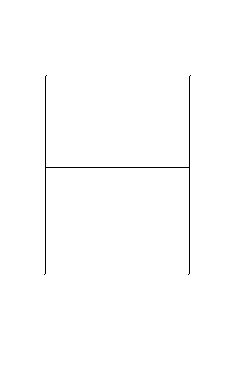
\includegraphics[width=.2\linewidth]{images/h-skel-inv}};
		\draw[->, ultra thick] (h0.east) to (h1.west);
	\end{tikzpicture}
%	}
	
	\vspace{0.5em}
	\caption{
		\emph{Skeletonisation} processes a binary image by converting regions of arbitrary thickness into 1-pixel thick paths, preserving 8-wise connectivity.
		\label{fig:skel}
	}
\end{figure}

\Cref{alg:paths} then uses these keypoints to detect and label paths within components.
Per component, a depth-first traversal is performed to discover the paths between all constituent interest points (\cref{alg:glyphgraph:dft}); this traversal prioritises moves to regular pixels over interest points, allowing interest points to be revisited since a path may start and end at the same point.
In \cref{alg:glyphgraph:ipan}, these paths are then subdivided using \citeauthor{PathCurvature}'s IPAN algorithm \cite{PathCurvature} to detect locations of high curvature (using the default parameters provided in the paper).
This is a two-pass approach, first testing each point $p$ along a path for the existence of an \emph{admissible} triangle built from $p$, one point preceding $p$, and one point succeeding $p$ in the path---these points must be within a distance range from $p$, and the internal angle $\alpha$ at $p$ must be sufficiently small.
If such a triangle exists, $p$ is marked as \emph{high-curvature} and its \emph{sharpness} $\pi - |\alpha|$ is recorded.
These locations are then refined by performing non-maximal suppression with the observed sharpness values, leaving only the local maxima marked as splitting points.

\Crefrange{alg:glyphgraph:split-start}{alg:glyphgraph:split-end} then classify each path segment: if for a path segment with length $t$ and distance $d$ between that segment's endpoints $d * \mathit{curve\_thres} < t$, then we label it as a \texttt{CURVE}, otherwise it is labelled as a \texttt{LINE}.
I consider $\mathit{curve\_thres} = 1.5$ as the default value.
An edge is then added to the graph between these two points, with the given label---modelling path curvature features as desired.

To establish and model orientation, \cref{alg:north} inserts a new vertex at $(0,0)$, and places an edge between this vertex and the closest interest point found in the image with a unique \texttt{NORTH} label.
\Cref{alg:neighbours} then captures the topological relationship between components.
Per-component, $\mathit{eps}$ is chosen to be either the set of that component's endpoints, keypoints or its sole start point (in decreasing order of preference).
An edge, labelled \texttt{NEIGHBOUR}, is then placed between each point in $\mathit{eps}$ and the nearest interest point in another component.
Note that when outputting the final graph, vertex position data is discarded with the goal of providing scale-invariance.

%?? Graph gen algo -- kinda explain this guy's path splitting algo \cite{PathCurvature}

\paragraph{An example walkthrough}
%?? High-level diagram, walkthrough (like the example in the proposal) -- do theta instead?
Consider a rough visual example aided by \cref{fig:walkthrough}---the transformation of an image of the character ``$\Theta$'' into a graph.
Firstly, our image (\cref{fig:walkthrough:glyph}) undergoes preprocessing and skeletonisation to capture the glyph's paths (\cref{fig:walkthrough:skel}).
This binary skeleton then undergoes connected component labelling, and the algorithm  identifies two main components present in the image: an outer oval component (orange), and an inner line component (red) (\cref{fig:walkthrough:comp}).

Each pixel is then examined and is classified as either an endpoint, keypoint or regular pixel according to its neighbourhood (\cref{fig:walkthrough:interest}).
The line component here features two endpoints, which are detected from their neighbourhoods.
In contrast, within the oval component every pixel has two contiguous blocks within its $3\times3$ neighbourhood, and so all are deemed to be ``regular''.

Paths between keypoints within each component are then traced out labelled to produce the first set of edges (\cref{fig:walkthrough:traversal}).
The inner component is traversed simply, starting at the left endpoint and ending at the right---the path is not split any further, and is classified as a \texttt{LINE}.
As the outer component has no interest points, traversal begins at the leftmost point on its top row, before moving clockwise.
Once the procedure returns to the start-point the IPAN algorithm is run on the traced path, which identifies a location of high curvature on the underside of the oval: creating a new vertex and two path segments.
As the path length for each segment is sufficiently larger than the distance between its endpoints, each is classified as a \texttt{CURVE}.

The final graph (\cref{fig:walkthrough:graph}) is produced by considering how these components relate to one another.
To capture the glyph's orientation, a purely logical vertex at $(0,0)$ is defined with no connection to any image component: a new edge is then placed between the logical vertex and the vertex on the top-side of the oval, its nearest neighbour, labelled as a \texttt{NORTH} relation.
Finally, we consider topological relationships: the endpoints of the inner component connect to their closest neighbour in the outer component with a \texttt{NEIGHBOUR} relation.
The reverse also occurs from the vertices in the outer component towards the inner, but duplicate \texttt{NEIGHBOUR} relationships are not stored.

\begin{figure}
	\def\pixels{
		{0,0,0,0,0,0,0,0,0,0,0},
		{0,0,0,0,1,1,1,0,0,0,0},
		{0,0,0,1,0,0,0,1,0,0,0},
		{0,0,1,0,0,0,0,0,1,0,0},
		{0,0,1,0,0,0,0,0,1,0,0},
		{0,0,1,0,1,1,1,0,1,0,0},
		{0,0,1,0,0,0,0,0,1,0,0},
		{0,0,1,0,0,0,0,0,1,0,0},
		{0,0,0,1,0,0,0,1,0,0,0},
		{0,0,0,0,1,1,1,0,0,0,0},
		{0,0,0,0,0,0,0,0,0,0,0}%
	}
	\def\comps{
		{0,0,0,0,0,0,0,0,0,0,0},
		{0,0,0,0,2,2,2,0,0,0,0},
		{0,0,0,2,0,0,0,2,0,0,0},
		{0,0,2,0,0,0,0,0,2,0,0},
		{0,0,2,0,0,0,0,0,2,0,0},
		{0,0,2,0,3,3,3,0,2,0,0},
		{0,0,2,0,0,0,0,0,2,0,0},
		{0,0,2,0,0,0,0,0,2,0,0},
		{0,0,0,2,0,0,0,2,0,0,0},
		{0,0,0,0,2,2,2,0,0,0,0},
		{0,0,0,0,0,0,0,0,0,0,0}%
	}
	\definecolor{pixel 0}{HTML}{FFFFFF}
	\definecolor{pixel 1}{HTML}{000000}
	\definecolor{pixel 4}{RGB}{150,227,240}%{HTML}{ff0000}
%	\definecolor{pixel 3}{RGB}{250,71,37}%{HTML}{00ff00}
	\colorlet{pixel 3}{uofglavendar}
%	\definecolor{pixel 2}{RGB}{253,161,77}%{HTML}{0000ff}
	\colorlet{pixel 2}{uofgpumpkin}%sunshine}
	\centering
	\begin{subfigure}[t]{0.3\linewidth}
		\resizebox{\linewidth}{!}{
		\begin{tikzpicture}
			\node[font=\fontsize{120}{120}\selectfont, draw] at (0,0) (Letter) {$\Theta$};
		\end{tikzpicture}
		}
		\caption{Glyph Image\label{fig:walkthrough:glyph}}
	\end{subfigure}
	~
	\begin{subfigure}[t]{0.3\linewidth}
		\resizebox{\linewidth}{!}{
		\begin{tikzpicture}
			\foreach \line [count=\y] in \pixels {
				\foreach \pix [count=\x] in \line {
					\draw[fill=pixel \pix] (\x,-\y) rectangle +(1,1);
				}
			}
		\end{tikzpicture}
		}
		\caption{Skeleton Image\label{fig:walkthrough:skel}}
	\end{subfigure}
	~
	\begin{subfigure}[t]{0.3\linewidth}
		\resizebox{\linewidth}{!}{
		\begin{tikzpicture}
			\foreach \line [count=\y] in \comps {
				\foreach \pix [count=\x] in \line {
					\draw[fill=pixel \pix] (\x,-\y) rectangle +(1,1);
				}
			}
		\end{tikzpicture}
		}
		\caption{Labelled Components\label{fig:walkthrough:comp}}
	\end{subfigure}
	~
	\begin{subfigure}[t]{0.3\linewidth}
		\centering
		\resizebox{\linewidth}{!}{
			\begin{tikzpicture}
			\foreach \line [count=\y] in \comps {
				\foreach \pix [count=\x] in \line {
					\draw[fill=pixel \pix!40!white] (\x,-\y) rectangle +(1,1);
				}
			}
			
			\node[draw, circle, color=black, fill=pixel 3, inner sep=0pt, minimum size=1.5cm, ultra thick] (n2) at (5.5,-5.5) {};
			\node[draw, circle, color=black, fill=pixel 3, inner sep=0pt, minimum size=1.5cm, ultra thick] (n3) at (7.5,-5.5) {};
			\end{tikzpicture}
		}
		\caption{Interest Points\label{fig:walkthrough:interest}}
	\end{subfigure}
	~
	\begin{subfigure}[t]{0.3\linewidth}
		\centering
		\resizebox{\linewidth}{!}{
			\large
			\begin{tikzpicture}[scale=0.5]
%			\foreach \line [count=\y] in \comps {
%				\foreach \pix [count=\x] in \line {
%					\draw[fill=pixel \pix!40!white] (\x,-\y) rectangle +(1,1);
%				}
%			}
		
			\node[draw, circle, color=black, fill=pixel 2] (n0) at (5.5,-1.5) {};
			\node[draw, circle, color=black, fill=pixel 2] (n1) at (6.5,-9.5) {};
			
			\node[draw, circle, color=black, fill=pixel 3] (n2) at (4.5,-5.5) {};
			\node[draw, circle, color=black, fill=pixel 3] (n3) at (7.5,-5.5) {};
			
			\draw[-, ultra thick] (n0) to [bend right=90] node [midway, fill=white] {2} (n1);
			\draw[-, ultra thick] (n0) to [bend left=90] node [midway, fill=white] {2} (n1);
			
			\draw[-, ultra thick] (n2) to node [midway, fill=white] {1} (n3);
			\end{tikzpicture}
		}
		\caption{Path Traversal and Splitting\label{fig:walkthrough:traversal}}
	\end{subfigure}
	~
	\begin{subfigure}[t]{0.3\linewidth}
		\resizebox{\linewidth}{!}{
		\large
		\begin{tikzpicture}[scale=0.5]
		%			\foreach \line [count=\y] in \comps {
		%				\foreach \pix [count=\x] in \line {
		%					\draw[fill=pixel \pix!40!white] (\x,-\y) rectangle +(1,1);
		%				}
		%			}
		
		\node[draw, circle, color=black, fill=white] (north) at (3,-1) {};
		\node[draw, circle, color=black, fill=pixel 2] (n0) at (5.5,-1.5) {};
		\node[draw, circle, color=black, fill=pixel 2] (n1) at (6.5,-9.5) {};
		
		\node[draw, circle, color=black, fill=pixel 3] (n2) at (4.5,-5.5) {};
		\node[draw, circle, color=black, fill=pixel 3] (n3) at (7.5,-5.5) {};
		
		\draw[-, ultra thick] (north) to node [midway, fill=white] {4} (n0);
		
		\draw[-, ultra thick] (n0) to [bend right=90] node [midway, fill=white] {2} (n1);
		\draw[-, ultra thick] (n0) to [bend left=90] node [midway, fill=white] {2} (n1);
		
		\draw[-, ultra thick] (n2) to node [midway, fill=white] {1} (n3);
		
		
		\draw[-, ultra thick] (n0) to node [midway, fill=white] {3} (n2);
		\draw[-, ultra thick] (n3) to node [midway, fill=white] {3} (n1);
		\end{tikzpicture}
		}
		\caption{Final Graph\label{fig:walkthrough:graph}}
	\end{subfigure}

	\vspace{0.5em}

	\caption{
		Walkthrough of $\Theta$'s image$\rightarrow$graph transformation by \texttt{GlyphGraph}.
		Labels have been simplified: $\mathtt{LINE}=1$, $\mathtt{CURVE}=2$, $\mathtt{NEIGHBOUR}=3$, $\mathtt{NORTH}=4$.
		Note that the downsampling observed here between \cref{fig:walkthrough:glyph,fig:walkthrough:skel} is \emph{not} part of the algorithm, and is performed only to aid understanding.
		\label{fig:walkthrough}}
\end{figure}

\paragraph{``Indistinct'' characters}
%?? Give example of (and explain) Z, H, K isomorphism in this scheme
When working with character images derived from fonts, \texttt{GlyphGraph} produces isomorphic graphs for characters which humans would instantly describe as distinct.
As shown by \cref{fig:badisomorphism} for the DejaVu Sans font, due to unexpected ``tails'' and conjunctions within the binary skeletons the letters `Z', `H' and `K' are jointly isomorphic.
What additional information exists within the structure of these characters that can be used to make their graphs more distinct?
By looking at the skeletonised forms alongside the output graph, the current modelling technique allows us to see features of glyph paths which might be used---in particular, we might wish to include positional data or the relative angle between lines and curves at interest points.
The first of these options likely comes at the cost of skew- or scale-invariance, but adapting \cref{alg:glyphgraph} to capture the latter class of features seems a worthwhile approach.

\begin{figure}
%	\definecolor{node}{RGB}{250,71,37}
	\colorlet{node}{uofgpumpkin}
	\centering
	\resizebox{0.8\linewidth}{!}{
		\Large
	\begin{tikzpicture}
		\node[draw](h0) at (0,0) {\includegraphics[width=.2\linewidth]{../imgs/dejavu-sans/H-Up}};
		\node[draw](k0) at (0,-3.5) {\includegraphics[width=.2\linewidth]{../imgs/dejavu-sans/K-Up}};
		\node[draw, label=below:{Glyphs}](z0) at (0,-7) {\includegraphics[width=.2\linewidth]{../imgs/dejavu-sans/Z-Up}};
		
		\node[draw](h1) at (4,0) {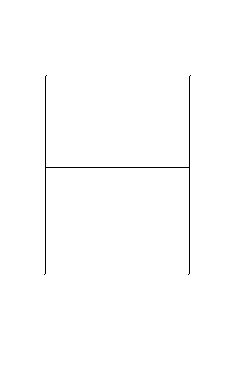
\includegraphics[width=.2\linewidth]{images/h-skel-inv}};
		\node[draw](k1) at (4,-3.5) {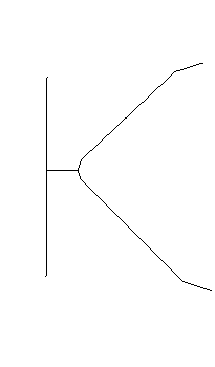
\includegraphics[width=.2\linewidth]{images/k-skel-inv}};
		\node[draw, label=below:{Skeletons}](z1) at (4,-7) {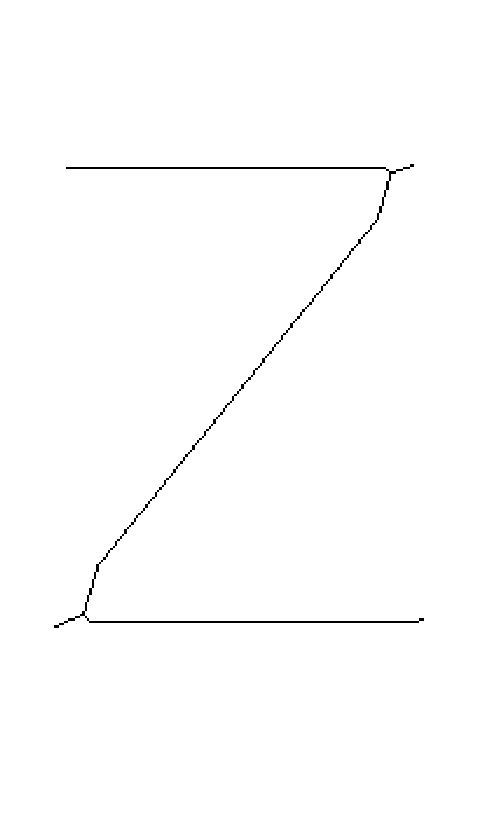
\includegraphics[width=.2\linewidth]{images/z-skel-inv}};
		
		\node[draw, circle, color=black, fill=white] (north) at (7,0) {};
		\node[draw, circle, color=black, fill=node] (n0) at (8,-2) {};
		\node[draw, circle, color=black, fill=node] (n1) at (8,-4) {};
		\node[draw, circle, color=black, fill=node] (n2) at (8,-6) {};
		\node[draw, circle, color=black, fill=node] (n3) at (10,-2) {};
		\node[draw, circle, color=black, fill=node] (n4) at (10,-4) {};
		\node[draw, circle, color=black, fill=node] (n5) at (10,-6) {};
		
		\draw[-, ultra thick] (north) to node [midway, fill=white] {4} (n0);
		\draw[-, ultra thick] (n1) to node [midway, fill=white] {1} (n0);
		\draw[-, ultra thick] (n1) to node [midway, fill=white] {1} (n2);
		\draw[-, ultra thick] (n1) to node [midway, fill=white] {1} (n4);
		\draw[-, ultra thick] (n4) to node [midway, fill=white] {1} (n3);
		\draw[-, ultra thick] (n4) to node [midway, fill=white] {1} (n5);
		
		\draw[->, ultra thick] (h0.east) to (h1.west);
		\draw[->, ultra thick] (k0.east) to (k1.west);
		\draw[->, ultra thick] (z0.east) to (z1.west);
		
		\draw[->, ultra thick] (h1.east) to ($(h1.east) + (1.5,-1)$);
		\draw[->, ultra thick] (k1.east) to ($(k1.east) + (1.5,0)$);
		\draw[->, ultra thick] (z1.east) to ($(z1.east) + (1.5,1)$);
		
		\node at (9,-7) {Output Graph};
	\end{tikzpicture}
	}
	
	\vspace{0.5em}
	
	\caption{Characters with isomorphic structure, which are thus ``identical'' \texttt{GlyphGraph} models.\label{fig:badisomorphism}}
\end{figure}

%\paragraph{An algorithm using path direction}
\subsection{A ``dual'' representation with path direction} \label{sec:algorithm:dual}
%?? introduce the ``dual'' representation (frame it like ``the graph models allowed me to learn \emph{why} these characters weren't distinct, and modify the algorithm to include path angle dynamics'')
In the framework established, it is difficult to capture the relationship between paths since they are modelled by edges.
To rework the model and enable these relationships to be captured, I start with a \emph{dual graph}-like conversion: edges in the prior model are converted into identically labelled vertices, placing an edge between these new vertices for each time their corresponding prior edges meet at the same vertex.
While this decision appears sensible since these labels \emph{are} the features recognised, to measure (and record) relative path angles it is insufficient to consider this transformation alone---\cref{alg:glyphgraph} measures and uses the start and end direction of each path segment, but these are not output.
A modification of the initial algorithm is thus required.

First we must divide our labellings into two classes: \emph{standard} features (lines and paths) which have well-defined directions at either end, and \emph{special} features (neighbourhood, north) which do not.
In the dual representation, edges between special$\leftrightarrow$regular edges are simply labelled `8' and special$\leftrightarrow$special edges are labelled `0'; the directional information becomes useful when considering regular$\leftrightarrow$regular relationships.
These directions are an integer in the range 0--7, numbering the neighbourhood pixels around a path's endpoint clockwise from north, and are assigned based on the location of the first point adjacent to that endpoint.
If two paths meet at a vertex, having directions $d$ and $d'$ at that point respectively, then their relationship is labelled $|d-d'|$.
Quite usefully, we \emph{can} return to the initial class of model from this new representation: each dual-vertex is transformed to an edge between two unknown vertices, which may be gradually inferred by iterating over the set of edges in the dual graph.
\Cref{fig:dual} shows the dual transformation of the regular model of `$\Theta$' from \cref{fig:walkthrough}.

%?? changes core model -- MCS is now effectively ``edge-maximising'' relative to our prior model.
Theoretically, this new approach should increase matching performance.
The MCS procedure as I have defined it maximises the order of the produced common subgraph, yet the features in my first model lie on the edges.
Running this procedure on a dual graph-like transformation gives similar results to the \emph{maximum common edge subgraph} of the regular model, matching in a way that puts more emphasis on the count of features between a pair of graphs.

\begin{figure}
	\centering
%	\resizebox{!}{4cm}{
	\begin{tikzpicture}
	\begin{scope}[auto, every node/.style={draw,circle,minimum size=2em,inner sep=1},node distance=2cm]
%	\node (n0) at (0,0) {4};
%	\node[fill=uofgpumpkin] (n1) at (2,0) {2};
%	\node[fill=uofgpumpkin] (n2) at (0,-2) {2};
%	\node (n3) at (2,-2) {3};
%	
%	\node[fill=uofglavendar, text=white] (n4) at (3,-3) {1};
%	\node (n5) at (4,-4) {3};
%	\node[fill=uofglavendar, text=white] (n4) at (4,-2) {1};
%	\node (n5) at (6,-2) {3};
	\node (n0) at (0,0) {4};
	\node[fill=uofgpumpkin] (n1) at (1.4,1.4) {2};
	\node[fill=uofgpumpkin] (n2) at (1.4,-1.4) {2};
	\node (n3) at (2.8,0) {3};
	
	\node[fill=uofglavendar, text=white] (n4) at (4.8,0) {1};
	\node (n5) at (6.8,0) {3};
	\end{scope}
	
	\draw[-, ultra thick] (n0) to node [midway, fill=white] {8} (n1);
	\draw[-, ultra thick] (n0) to node [midway, fill=white] {8} (n2);
	\draw[-, ultra thick] (n0) to node [near end, fill=white] {0} (n3);
	
	\draw[-, ultra thick] (n1) to node [near end, fill=white] {3,4} (n2);
	\draw[-, ultra thick] (n1) to node [midway, fill=white] {8} (n3);
	
	\draw[-, ultra thick] (n2) to node [midway, fill=white] {8} (n3);
	
	\draw[-, ultra thick] (n3) to node [midway, fill=white] {8} (n4);
	
	\draw[-, ultra thick] (n4) to node [midway, fill=white] {8} (n5);
	
%	\draw[-, ultra thick] (n2) to [bend right=60] node [midway, fill=white] {8} (n5);
%	\draw[-, ultra thick] (n1) to [bend left=60] node [midway, fill=white] {8} (n5);
	\draw[-, ultra thick] (n2) to [bend right=30] node [midway, fill=white] {8} (n5);
	\draw[-, ultra thick] (n1) to [bend left=30] node [midway, fill=white] {8} (n5);
	\end{tikzpicture}
%	}
	
	\vspace{0.5em}
	\caption{
		The dual graph of \emph{`$\Theta$'}, with path features coloured to match their parent component in \cref{fig:walkthrough:graph}.
		Node labels here match \cref{fig:walkthrough}'s shorthand for features, where edge labels denote relative path angles.
		Note that both `2' edges in the regular representation start and meet at the same point, and thus have two relative angles against each other in the glyph.
		\label{fig:dual}
	}
\end{figure}

%?? old model is recoverable from new.

%====================================================
\section{Modifications to k-Down}
\label{sec:k-down-mods}
%====================================================

%?? Why? Attributed multi-graphs
Having seen that both of the proposed models take the form of attributed multigraphs, \citeauthor{Between-MCS-SIP}'s $k\downarrow$ requires adaptation to accommodate graphs as I have defined them.
%?? Discuss/introduce $s$-adjacency (Already added $N^{=}_{s},N^{\succcurlyeq}_{s}$ to graph definitions section), and 3 levels of filtering (induced, edge-count-increasing, barely overlapping)
The first step in matching these graphs is to determine which sequence-aware neighbourhood (and thus adjacency operator) will be used to impose the constraints arising from edge labels.
Each corresponds to a different level of filtering:
\begin{itemize}
	\item the exact neighbourhood $N^{=}_{s,\mathcal{G}}$ is necessary in the \emph{induced} variant of MCS, so that a pair of pattern and target vertex pairs may only map to one another if they have identical edge sequences;
	
	\item the overlap neighbourhood $N^{\circ}_{s,\mathcal{G}}$ provides the bare-minimum level of filtering needed when considering the \emph{non-induced} variant of MCS, allowing a pair of pattern and target vertex pairs to map to one another if there is any overlap in the edge sequences;
	
	\item the sufficient neighbourhood $N^{\succcurlyeq}_{s,\mathcal{G}}$, which allows a pattern vertex pair to be mapped to a target vertex pair if every edge in the former can be mapped to an edge of equal value in the latter, offering an oddly asymmetrical mapping when used in MCS---I define this (in the context of SIP) as building an \emph{edge-count-increasing subgraph isomorphism}.
\end{itemize}

\Cref{alg:k-down-search} then defines the necessary modifications to $k\downarrow$ to compute the MCS in each case.
%?? Filtering at top of search---modify loop constraints, vertex label matching
At the top of search, the matching procedure must enforce that vertices of $\mathcal{P}$ can only be mapped to vertices of $\mathcal{T}$ with equal labels.
Additionally, any vertices featuring loops must meet the selected sequence-adjacency criterion (\crefrange{alg:k-down-search:top-start}{alg:k-down-search:top-end}).
%?? Per-node of search, look at $s$-neighbourhoods
Per node of constraint propagation, domains are pruned using the chosen sequence-aware neighbourhood---if $v$ is mapped to $v'$ and $v$ and $w$ are adjacent with edge sequence $s$ in $\mathcal{P}$, then $w$ may only be assigned to vertices in the $s$-neighbourhood of $v'$ (\crefrange{alg:k-down-search:node-start}{alg:k-down-search:node-end}).

%?? Keep standard filtering from supplemental graphs (adjacency matrix operates on at least 1-adjacency, exact matches are provided)
The rest of the algorithm is unaffected by these additions; by providing both multigraph and simple graph notions of neighbourhood and adjacency, the existing filtering provided by supplemental graphs is maintained.
%?? Could use path-based inference for new supplemental graphs, but probably way too much work for graphs of this order (i.e.\ very small)
Admittedly, further supplemental graphs could be added, filtering on commonly seen label patterns in paths; although with the relatively low-order graphs produced by the examined models such optimisations would be largely unnecessary for this study.

\begin{algorithm}[t]
	\DontPrintSemicolon
	\caption{Modifications to k$\downarrow$ \cite{Between-MCS-SIP} for attributed multigraphs, given (for a graph $\mathcal{G}$) a vertex labelling function $\ell_\mathcal{G}$, a chosen multigraph neighbourhood function $\mathcal{N}_{s,\mathcal{G}}$ and its associated adjacency operator ``$\sim_{s,\mathcal{G}}$''. \label{alg:k-down-search}}
	\tcp{
%		replacement for lines 5--9\\
		top-of-search filtering with sequences on loop constraints}
	\ForEach{$v \in \operatorname{V}(\mathcal{P})$}{
		$D_v \leftarrow \operatorname{V}(\mathcal{T})$\;
		\ForEach{$(P,T)\in L$}{
			$D_v \leftarrow \{ w \in D_v : v \sim_P v \Rightarrow w \sim_T w \land S_P(v) \lesspreceq{k} S_T(w) \}$
		}
	
		\BlankLine
		$s \leftarrow \operatorname{seq}_{\mathcal{P}}(v,v)$\;\label{alg:k-down-search:top-start}
%		$Valids \leftarrow \{\}$\;
%		\ForEach{$w \in \operatorname{V}(\mathcal{T})$}{
%			\If{$v \sim_{\mathcal{P}} v \Rightarrow w \sim_{s,\mathcal{T}} w \land l_\mathcal{P}(v) = l_\mathcal{T}(w)$}{
%				$Valids \leftarrow Loops \cup \{w\}$
%			}
%		}
		$D_v \leftarrow \{ w \in D_v : \ell_\mathcal{P}(v) = \ell_\mathcal{T}(w) \land v \sim_P v \Rightarrow w \sim_{s,\mathcal{T}} w \}$\;\label{alg:k-down-search:top-end}
		$D_v \leftarrow D_v \cup k$ distinct wildcard vertices\;
	}
	
	\BlankLine
	\BlankLine
	\tcp{
%		replacement for lines 35--40\\
	filtering with sequences during propagation}
	\ForEach{$D_w \in D\backslash\lbrace D_v\rbrace$}{
		$D_w \leftarrow D_w \backslash \lbrace v'\rbrace$\;
		\ForEach{$(P, T) \in L$}{
			\If{$v \sim_P w$}{
				$D_w \leftarrow D_w \cap (N_T(v') \cup \mathit{wildcards} )$
			}
		}
		\BlankLine
		$(P_0, T_0) \leftarrow L[0] $\;\label{alg:k-down-search:node-start}
		\If{$v \sim_{P_0} w$}{
			$s \leftarrow \operatorname{seq}_{P_0}(v,w)$\;
			$D_w \leftarrow D_w \cap (\mathcal{N}_{s,T_0}(v') \cup \mathit{wildcards} )$\;\label{alg:k-down-search:node-end}
		}
		\If{$D_w = \emptyset$}{\Return{\textbf{false}}}
	}
\end{algorithm}

%====================================================
\section{Experimental Evaluation} % \& Discussion}
\label{sec:evaluation}
%====================================================

To test the effectiveness of these algorithms for character modelling and classification, three experiments were performed:

%?? Describe your experiments. What criteria makes them successful/a good outcome? MAKE THIS CLEAR.

%?? Explain methodology

\begin{enumerate}
	\item Firstly, it is necessary to determine whether these graph models allow matching of characters formed in distinct, uniform, machine-generated styles.
	This is explored via the construction of ``confusion matrices'' between all graphs of characters in the Latin alphabet from several fonts, both lower- and upper-case.
	To this end, the order of the maximum common subgraph and graph edit distance are displayed via heat-maps to show character graph (dis-)similarity within and between fonts.
	For this, I chose three fonts to investigate: \emph{DejaVu Sans}, \emph{Open Sans} (both sans-serif), and \emph{Alegreya} (serif).
	The aim is to show that the generated graphs are reasonably distinct from one another within a human definition of similarity (i.e.\ we might expect 'o' and 'O' to produce identical graphs).
	Furthermore, I investigate whether the modifications introduced in \cref{sec:algorithm:dual} create more distinct glyph models as hypothesised.
	The experiment is judged to be a success if most character pairs do not exhibit isomorphism within each font, having a GED close to the median graph size.
	Naturally, a character will be isomorphic to itself \emph{within} a font, and thus another success criterion is that its model is ideally similar to the graph model of that same character from another font.
	
	\item To determine how well these models capture core character features between different styles of writing, I apply a \emph{$k$-Nearest Neighbours} ($k$NN) classifier to the HWRT database of online handwritten character data \cite{HwrtDatabase} (setting $k=5$ as in \cite{Graphs-Handwriting}).
	Images (and graphs) were constructed from the online path data using a selection of pen-radii, for $r \in \{1,5,9\}$, to explore how different levels of connectivity would affect graph structure and matching accuracy.
	Specifically, this online data decomposes paths into positions on a canvas with attached timestamps: images were reconstructed by applying Bresenham's line algorithm between these path points, generating a list of locations to place a circle of thickness $r$.
	For this classifier graph edit distance is the chosen metric, setting a timeout of \SI{30}{\second} per graph comparison.
	Due to the vast size of the dataset I restrict the database to the set of upper-case Latin alphabet characters, using a total of 2000 randomly selected glyphs split into \emph{test} and \emph{training} data
	As the database is already divided into a test and training set, I take subsets of each maintaining the existing proportion.
	This experiment assesses whether the features captured within any glyph were consistent between similar images in a way that enabled optical character recognition---a sufficiently high accuracy ($\sim\SI{90}{\percent}$) would indicate success.
	
	\item Finally, it is important to position this work in relation to existing graph models which have been applied to handwritten word recognition.
	For this task, I apply the same classifier to a subset of the George Washington Letters dataset\footnote{\url{http://histograph.ch}} made available by \citeauthor{Graphs-Handwriting} \cite{Graphs-Handwriting}.
	I use the same parameters on the classifier ($k=5$, \SI{30}{\second} timeout).
	Additionally, I attempt to explore how variation of the path curvature threshold during modelling affects classifier performance, examining $\mathit{curve\_thres} \in \{1.2, 1.35. 1.5, 1.65\}$.
	This experiment allows me to directly compare the modelling efficiency of my graph models combined with the defined GED against \citeauthor{Graphs-Handwriting}'s existing modelling techniques.
	As these graphs model whole words, graph order is likely to become an issue, harming classifier performance---made aware of this, I consider a lower classifier performance ($\sim\SI{80}{\percent}$, roughly the result of \citeauthor{Graphs-Handwriting}) to be successful.
\end{enumerate}

\noindent
All experiments were run on a Windows 10 Pro x64 machine using the Windows Subsystem for Linux, with an Intel Core i7--920@\SI{2.67}{\GHz} and \SI{12}{\gibi\byte} RAM.
All code used for these experiments is publicly accessible on GitHub\footnote{\url{https://github.com/FelixMcFelix/sip-for-cv-paper}}.
In all cases, statistics on generated graph order and size were collected in \cref{tab:graphstats}, allowing further commentary on suspected reasons behind matching performance.
Similarly, each experiment was attempted at all levels of filtering defined in \cref{sec:k-down-mods} to determine the related effects of each on classifier performance.

%?? Machine statistics, find the code here\footnote{\url{https://github.com/FelixMcFelix/sip-for-cv-paper}}, roll up a nice VM for review?

?? SET UP VM!

\subsection{Results and Discussion}

% disable these diagrams temporarily
%\renewcommand{\includestandalone}[3]{}%\includegraphics[width=\linewidth]{#1.png}}
\DeclareDocumentCommand\includestandalone{oom}{\includegraphics[width=\linewidth]{#3.png}}

\begin{figure*}
	\centering
	\begin{subfigure}[b]{0.3\linewidth}
		\includestandalone[width=\linewidth]{../tables/dejavu-sans/induced-conf-nrm}
		\caption{
			Induced
			\label{fig:heat:filter:induced}
%			goop monster quest?
		}
	\end{subfigure}
	\begin{subfigure}[b]{0.3\linewidth}
		\includestandalone[width=\linewidth]{../tables/dejavu-sans/edgecountinc-conf-nrm}
		\caption{
			Edge-count-increasing
			\label{fig:heat:filter:eci}
%			smile!
		}
	\end{subfigure}
	\begin{subfigure}[b]{0.3\linewidth}
		\includestandalone[width=\linewidth]{../tables/dejavu-sans/edgecountdec-conf-nrm}
		\caption{
%			yes!
			Non-Induced
			\label{fig:heat:filter:non-ind}
		}
	\end{subfigure}

\vspace{0.5em}
\caption{
	%goop monster quest? smile! yes!
	Heatmaps displaying graph similarity (graph order of MCS) between glyph graphs in the DejaVu Sans typeface, normalised by the order of the largest graph in the comparison.
	These plots show the effects of the different levels of filtering introduced in \cref{sec:k-down-mods}.
	Warmer colours imply more similarity, where cream means isomorphism---an overall darker heatmap shows that characters are seen as more distinct when matching under the given filtering level.	
	It can thus be seen that characters are perceived as being more distinct when computing the  induced MCS.
	\label{fig:heat:filter}
}
\end{figure*}

\begin{figure*}
	\centering
	\begin{subfigure}[b]{0.225\linewidth}
		\includestandalone[width=\linewidth]{../tables/dejavu-sans/induced-conf-nrm}
		\caption{MCS: Regular\label{fig:heat:dual:mcs-r}}
	\end{subfigure}
	\begin{subfigure}[b]{0.225\linewidth}
		\includestandalone[width=\linewidth]{../tables/dual-dejavu-sans/induced-conf-nrm}
		\caption{MCS: Dual\label{fig:heat:dual:mcs-d}}
	\end{subfigure}
	\begin{subfigure}[b]{0.225\linewidth}
		\includestandalone[width=\linewidth]{../tables/dejavu-sans/induced-conf-ged}
		\caption{GED: Regular\label{fig:heat:dual:ged-r}}
	\end{subfigure}
	\begin{subfigure}[b]{0.225\linewidth}
		\includestandalone[width=\linewidth]{../tables/dual-dejavu-sans/induced-conf-ged}
		\caption{GED: Dual\label{fig:heat:dual:ged-d}}
	\end{subfigure}
	
	\vspace{0.5em}
	\caption{
		Heatmaps displaying graph similarity (MCS) and dissimilarity (GED) in the DejaVu Sans typeface as in \cref{fig:heat:filter}, comparing the distinctiveness of character graphs from the `Regular' and `Dual' algorithm variants.
		For GED, lighter colours again imply similarity, where cream implies isomorphism---characters are more distinct in one encoding if lower similarity is observed outside of the diagonal.
		Crucially, we can see that the `Dual' encoding leads to more distinctive characters as expected.
		\label{fig:heat:dual}
	}
\end{figure*}

\begin{figure*}
	\centering
	\begin{subfigure}[b]{0.225\linewidth}
		\includestandalone[width=\linewidth]{../tables/open-sans-dejavu-sans/induced-conf-nrm}
		\caption{MCS: Regular\label{fig:heat:sans:mcs-r}}
	\end{subfigure}
	\begin{subfigure}[b]{0.225\linewidth}
		\includestandalone[width=\linewidth]{../tables/dual-open-sans-dejavu-sans/induced-conf-nrm}
		\caption{MCS: Dual\label{fig:heat:sans:mcs-d}}
	\end{subfigure}
	\begin{subfigure}[b]{0.225\linewidth}
		\includestandalone[width=\linewidth]{../tables/open-sans-dejavu-sans/induced-conf-ged}
		\caption{GED: Regular\label{fig:heat:sans:ged-r}}
	\end{subfigure}
	\begin{subfigure}[b]{0.225\linewidth}
		\includestandalone[width=\linewidth]{../tables/dual-open-sans-dejavu-sans/induced-conf-ged}
		\caption{GED: Dual\label{fig:heat:sans:ged-d}}
	\end{subfigure}
	
	\vspace{0.5em}
	\caption{
		Heatmaps displaying graph (dis-)similarity between the DejaVu Sans and Open Sans typefaces, conveyed as in \cref{fig:heat:dual}.
		Ideally, matching characters are expected to be almost isomorphic---high MCS order and low GED are expected along the diagonal.
		While some isomorphisms and general similarities per-character are preserved between fonts, many of these are lost.
		\label{fig:heat:sans}
	}
\end{figure*}

\begin{figure*}
	\centering
	\begin{subfigure}[b]{0.225\linewidth}
		\includestandalone[width=\linewidth]{../tables/alegreya-dejavu-sans/induced-conf-nrm}
		\caption{MCS: Regular\label{fig:heat:vs:mcs-r}}
	\end{subfigure}
	\begin{subfigure}[b]{0.225\linewidth}
		\includestandalone[width=\linewidth]{../tables/dual-alegreya-dejavu-sans/induced-conf-nrm}
		\caption{MCS: Dual\label{fig:heat:vs:mcs-d}}
	\end{subfigure}
	\begin{subfigure}[b]{0.225\linewidth}
		\includestandalone[width=\linewidth]{../tables/alegreya-dejavu-sans/induced-conf-ged}
		\caption{GED: Regular\label{fig:heat:vs:ged-r}}
	\end{subfigure}
	\begin{subfigure}[b]{0.225\linewidth}
		\includestandalone[width=\linewidth]{../tables/dual-alegreya-dejavu-sans/induced-conf-ged}
		\caption{GED: Dual\label{fig:heat:vs:ged-d}}
	\end{subfigure}
	
	\vspace{0.5em}
	\caption{
		Heatmaps displaying graph (dis-)similarity between the DejaVu Sans and Alegreya typefaces.
		Serif characters (such as those of Alegreya) modify many characters at the end of paths---ideally, core elements of the letter forms should remain identical.
		Criteria for analysis match those of \cref{fig:heat:sans}.
		Aside from `o', `O' and `Q', neither the `Regular' nor `Dual' graphs reliably enable matching between two different typeface styles.
		\label{fig:heat:vs}
	}
\end{figure*}

%?? EXPLAIN WHAT THE GRAPHS/MAPS SHOW, Discuss graph order in both cases. (min, max, median, avg)

%?? Heatmaps per font -- examine size? font v font? sans vs serif? Dual vs regular? How do the different filtering levels affect character distinctness? Use the word ``curiously'' to describe relation between more distinct chars and reduced classifier performance.
%
%?? Matching effectiveness statistics with HWRT \cite{HwrtDatabase} (Discuss effects of pen thickness, filtering class, dual vs regular). kNN classifier ($k=5$ I think) Have to reduce dataset size due to cost of evaluation -- full HWRT dataset means several billion graph comparisons. They're expensive!

%?? How long did these experiments take? Anywhere between seconds and minutes per query graph dependant on size of graphs, training data size (fast on alphabet 30 mins, slow on words ~??).

%?? What else? Try it out on the george washington letters dataset for direct comparison with \cite{Graphs-Handwriting}? IF NOT DONE, PUT IN FUTURE WORK\footnote{\url{http://histograph.ch}}

%?? Table with font graph stats
\begin{table}
	\centering
	
	\resizebox{\linewidth}{!}{
		\begin{tabular}{lccccccc}\toprule
			\multicolumn{1}{c}{Font} & \multicolumn{1}{c}{Model} & \multicolumn{3}{c}{Graph Order} & \multicolumn{3}{c}{Graph Size} \\
			& & Min & Max & Median & Min & Max & Median \\
			\midrule
			Alegreya & Regular & 2 & 26 & 11 & 2 & 25 & 11 \\
			& Dual & 2 & 25 & 11 & 3 & 37 & 14.5 \\
			DejaVu Sans & Regular & 2 & 14 & 6 & 2 & 13 & 6 \\
			& Dual & 2 & 13 & 6 & 1 & 14 & 7 \\
			Open Sans & Regular & 2 & 17 & 6 & 2 & 16 & 6 \\
			& Dual & 2 & 16 & 6 & 1 & 18 & 7 \\
			HWRT ($r=1$) & Regular & 2 & 113 & 7 & 2 & 172 & 6 \\
			& Dual & 2 & 172 & 6 & 1 & 398 & 8 \\
			HWRT ($r=5$) & Regular & 0 & 40 & 7 & 0 & 55 & 6 \\
			& Dual & 0 & 55 & 6 & 0 & 116 & 7\\
			HWRT ($r=9$) & Regular & 2 & 59 & 7 & 1 & 126 & 8 \\
			& Dual & 2 & 41 & 7 & 1 & 126 & 8 \\
			Washington & Regular & 7 & 75 & 33 & 6 & 93 & 42 \\
			& Dual & 6 & 93 & 42 & 6 & 170 & 75 \\
			\bottomrule
		\end{tabular}
	}
	
	\vspace{0.5em}
	\caption{
		Aggregate statistics on graph order and size produced from the used datasets.
		\label{tab:graphstats}
	}
\end{table}

\paragraph{Experiment 1}
\Cref{fig:heat:filter} shows the effect of each level of $k\downarrow$ filtering upon character distinctness during matching.
Few differences are noted between the edge-count-increasing and non-induced levels of filtering (\cref{fig:heat:filter:eci,fig:heat:filter:non-ind} respectively), likely as they both build on the use of the non-induced variant of MCS.
The induced MCS (\cref{fig:heat:filter:induced}), on the other hand, finds the set of characters to be largely more distinct from one another due to its stronger filtering.
A more thorough examination reveals that many sets of unexpected isomorphisms remain: \{Z, H, K\} as explained in \cref{fig:badisomorphism}, \{n, h\}, \{c, s, C, S\}, \{b, p\}, and \{q, d\} to name several.
While many of these are expected due to identical upper- and lower-case forms, several of these suggest that the original model lacks discriminative power and captures too few features; chiefly, these appear to be path length, path angle dynamics and glyph size.
Throughout all comparisons, it is clear that many of these graphs still exhibit high similarity to one another (\SIrange{60}{70}{\percent} in the induced case), implying that many of the character graphs share identical components.
This may arise from the fact that the MCS is not \emph{connected}, i.e. I do not impose that there must be a path between every pair of vertices in the MCS; this allows the addition of extra vertices which have no paths to the main components during matching.
For instance, in every graph an edge marked \texttt{NORTH} between a pair of vertices is guaranteed to exist, and during search may be added to the MCS ``for free'' if it is disconnected from the current incumbent.

Having established the induced variant of MCS as the most discriminative, \cref{fig:heat:dual} then presents the effects of the dual encoding upon glyph similarity for this level of filtering.
Broadly, \cref{fig:heat:dual:mcs-r,fig:heat:dual:mcs-d} show an overall reduction in similarity across the entire space of comparisons---showing that the dual graph representation is successful in making glyph models more distinct from one another.
Many of the unexpected isomorphisms \emph{have} been removed by this modification to the algorithm, yet not all; note that \{H, K\}, \{n, h\}, \{b, p\}, and \{q, d\} remain isomorphic, alongside many of the prior letters with ``identical'' upper- and lower-case forms.
While it is unsurprising that a few such isomorphisms remain (we have not yet modelled the phenomena which actually differentiate them), revisiting \cref{fig:badisomorphism} sheds some light on the case of `H' and `K'.
Note that in `K', the skeleton paths form then right junction start vertically leading to identical path dynamics between the two glyphs, which of course suggests further modifications which could be made to account for \emph{overall} path direction.
I do not consider further such modification here.

\Cref{fig:heat:sans,fig:heat:vs} then demonstrate the observed similarity \emph{between} fonts of different classes, examining DejaVu Sans vs.\ Open Sans and Alegreya respectively.
In the former case, while some portion of the expected isomorphisms were observed it is clear from the visual similarity of the fonts themselves that the model was unable to capture the core features that define many of the glyphs.
Somewhat interestingly, changing to the `Dual' encoding from \cref{fig:heat:sans:mcs-r} to \cref{fig:heat:sans:mcs-d} \emph{removed} some of these observed isomorphisms, indicating different curvature along the traversed paths.
Indeed, curvature may well be the root of many of the other `missing' isomorphisms, as path-splitting using the IPAN algorithm is likely to have some sensitivity to what humans might appreciate as minor variation.
In the case of DejaVu Sans against Alegreya, while some clear glyph isomorphisms are preserved between fonts (\{o, O\}, and `Q'), the font graphs exhibit startling dissimilarity.
A considerable factor here is the difference in graph order of these font classes; serif fonts display far more variation and ornamentation, particularly on what letter path endpoints.
This naturally leads to more paths between these points, leading to a rather different structure overall.
Given the nature of how \texttt{NEIGHBOURHOOD} and \texttt{NORTH} relations are formed, the existence of serifs further complicates matching as these relations are more likely in practice to concern endpoints.

While successful within a font, the overall results do not bode well---they indicate that the modelling techniques and/or the similarity measures are not fit for purpose when comparing writing in different styles or even regular variation within a single style.
Overall on the specified machine, these experiments typically took around \SI{30}{\minute} each to execute all $52\times52$ graph comparisons.

\paragraph{Experiment 2}
?? Accuracy statistics for Exp 2 ``Curiously, more distinct characters do not necessarily imply better matching performance''

\paragraph{Experiment 3}
?? Accuracy statistics for Exp 3

%\subsection{Discussion}
%
%?? Discuss Exp 1
%
%?? Discuss Exp 2
%
%?? Discuss Exp 3

%====================================================
\section{Related Work}
\label{sec:related}
%====================================================

\paragraph{General image modelling}
%?? GENERAL STUFF
Historically, the \emph{Scale-Invariant Feature Transform} (SIFT) and similar approaches have been extremely popular vector-space models for image modelling and matching \cite{SIFT,Sift-Variants-Comparison}.
These techniques typically operate by identifying locations of high variation within a multiscale representation of an image such as a \emph{Laplacian pyramid}, capturing high-dimensional gradient neighbourhoods of these points as features.
%Feature vectors are then histograms of gradient neighbourhoods, subject to preprocessing to identify the dominant direction and correct for variation in luminance, capturing distinctive image regions at different scales.
%These typically find uses in image matching (using the Hough transform) and panorama stitching (using RANSAC \cite{SIFT-Panorama})---since these are high-dimensionality keypoints, such matching can be expensive, motivating the development of cheaper (but less discriminative) models such as SURF \cite{SURF}.
%Adding to this, SIFT vectors have been used within complete graph topologies for the task of facial recognition \cite{SIFT-Graph-Topology-Faces}.

\emph{Convolutional neural networks} (CNNs) have been a sizeable area of focus recently, with approaches such as \citeauthor{ConvNet} \cite{ConvNet} proving able to accurately learn image labellings from large datasets.
These models operate by statistically learning \emph{kernels} from a corpus of training data to perform image convolution, transforming an image several times to eventually provide an output classification.
Given that these kernels are relatively high-dimensional vectors of real values, these are not typically transformations which can be intuited easily.
This reinforces the ``black-box'' nature of these models, and in combination with work on adversarial images \cite{AdversarialML} it is clear that the sensitivities and weaknesses of such models are extraordinarily difficult to estimate.
While complex networks can require a large volume of training data and have a costly training phase, CNNs achieve very high accuracy above and beyond existing vector-space models while having good performance on modern commodity hardware.
Primarily, this is due to the introduction of fast convolution operations on graphics processing units.
Notably, the cost of classification \emph{does not typically scale} with the size of the training data set, as the model learned is a \emph{fixed representation}.
Further advances by \citeauthor{MultilabelCNN} have extended such object classifiers with intelligent segmentation algorithms \cite{BING} to enable multiple labelling and accurate object location \cite{MultilabelCNN}.

%?? HANDWRITING STUFF

%\paragraph{Graph modelling of handwriting}
\paragraph{Handwriting and character recognition}
Techniques in this field are broadly split into two categories; \emph{online} classifiers use direct path input data as captured by a computer, and \emph{offline} classifiers which use image data (typically extracted from some real-world context).
Within this framework, the approach I have introduced and evaluated is an offline approach.

Currently, neural networks (both standard and convolutional) are a key model within offline recognition \cite{Handwriting-CNN-1,Handwriting-CNN-2}---able to tackle word recognition and spotting to high accuracy in different scripts and language datasets.
Aside from this, the use of SIFT-like keypoints for the task of offline Arabic word recognition has been successfully explored within a bag-of-features Hidden Markov Model \cite{Arabic-SIFT}, achieving a lower complexity (and similar effectiveness to) competing techniques.
This approach have been further applied to the task of word-spotting from the George Washington dataset \cite{Arabic-SIFT-Better}.

%?? Handwriting analysis w/ kNN \cite{Graphs-Handwriting}. How does their approach differ from mine? (Path curvature characteristics vs positional data)
Several existing approaches towards offline graph modelling of handwritten text are provided by \citeauthor{Graphs-Handwriting} \cite{Graphs-Handwriting}.
Their work focuses on analysis of the George Washington letters dataset by a $k$NN classifier using an approximate GED metric \cite{GED-Approx}.
In all cases, vertices are labelled with normalised $(\hat{x}, \hat{y})$ coordinates with edges left unlabelled.
The first of their approaches corresponds closely to my own---endpoints and junctions are identified within a skeletonised glyph image, and edges are placed by following paths and creating new vertices for every distance $d$ travelled.
Other approaches focus on grid-based segmentation (with edges provided through various techniques) and adaptive segmentations combined with edges from path traversal.
They find that the keypoint-based approach has \SI{77}{\percent} accuracy at the cost of very high graph order and size, while adaptive segmentations produce lower order graphs with higher ($\sim\SI{80}{\percent}$) accuracy.
Interestingly, they note that the use of the Delaunay triangulation for such models results in reduced classifier performance ($\sim\SI{63}{\percent}$) with the highest graph sizes, supporting my earlier findings in \cref{sec:image-weakness}.

%?? Discuss ML work on handwriting modelling and its effectiveness? Why is ML better here? Fixed execution time (irrespective of training set size), so benefits from extra training in a way 

%====================================================
\section{Further Applications}
\label{sec:applications}
%====================================================

?? Give example of graph of two circuit diagrams here

?? Examine graph order---too big? Can we run SIP on it? How are the results?

%====================================================
\section{Conclusions and Future Work}
\label{sec:conclusion}
%====================================================

?? Draw conclusions here---sum up paper.

?? WHY did it not work as planned? Growing execution time as training set sizes (since we are comparing against \emph{all} known entries) (choice of kNN as a classifier).

?? Downsides of approach? graph models seemingly need to be designed specifically for the task at hand (need an explicit notion of things and relationships)---whereas existing ML models are effective because they are designed to learn features of arbitrary high-dimensional data by statistics (in the case of CNNs/NNs, by learning parameters)

?? Final thought? needs total rework -- addition of more information/hacks appears good at first, then fails.

?? Perhaps it could be effective, when used with approximate GED... \cite{GED-Approx}

?? Future work? Approximate GED metrics? Investigation of path-based supplemental graphs?

?? MCS/GED bad fit? i.e. p,q,b,d have small GED since all that moves is the north relation. At that point, are we really performing graph matching?

?? Investigate more interesting side-constraints in search -- such as temporal subgraph ismoporhism \cite{TSIP-Long} (Explain briefly, then discuss why it might be useful? (patterns, not exact matching))

?? Graph order of GW data inhibits matching effectiveness. Investigate effect of adapting McSplit algorithm for this purpose? (only induced matching, but this is the best so yeah)

?? How might it handle fonts designed for OCR? font-sizes?

?? More general techniques? Multiscale feature graphs? (lol)

%====================================================
\noindent
{\bf Acknowledgements.}
%====================================================
I'd like to thank my supervisors Patrick Prosser, John Williamson and Ciaran McCreesh for their comments and guidance throughout the year.
I'd also like to thank my girlfriend Vanessa Stevenson and my family for their continued support.

%====================================================
\section{References}
%====================================================
\printbibliography[heading=none]

% Fix weird underhang of last reference
\vspace{1em}

\end{document}